\documentclass{sigchi}

% Use this section to set the ACM copyright statement (e.g. for
% preprints).  Consult the conference website for the camera-ready
% copyright statement.

% Copyright
\CopyrightYear{2016}
%\setcopyright{acmcopyright}
\setcopyright{acmlicensed}
%\setcopyright{rightsretained}
%\setcopyright{usgov}
%\setcopyright{usgovmixed}
%\setcopyright{cagov}
%\setcopyright{cagovmixed}
% DOI
\doi{http://dx.doi.org/10.475/123_4}
% ISBN
\isbn{123-4567-24-567/08/06}
%Conference
\conferenceinfo{CHI'16,}{May 07--12, 2016, San Jose, CA, USA}
%Price
\acmPrice{\$15.00}

% Use this command to override the default ACM copyright statement
% (e.g. for preprints).  Consult the conference website for the
% camera-ready copyright statement.

%% HOW TO OVERRIDE THE DEFAULT COPYRIGHT STRIP --
%% Please note you need to make sure the copy for your specific
%% license is used here!
% \toappear{
% Permission to make digital or hard copies of all or part of this work
% for personal or classroom use is granted without fee provided that
% copies are not made or distributed for profit or commercial advantage
% and that copies bear this notice and the full citation on the first
% page. Copyrights for components of this work owned by others than ACM
% must be honored. Abstracting with credit is permitted. To copy
% otherwise, or republish, to post on servers or to redistribute to
% lists, requires prior specific permission and/or a fee. Request
% permissions from \href{mailto:Permissions@acm.org}{Permissions@acm.org}. \\
% \emph{CHI '16},  May 07--12, 2016, San Jose, CA, USA \\
% ACM xxx-x-xxxx-xxxx-x/xx/xx\ldots \$15.00 \\
% DOI: \url{http://dx.doi.org/xx.xxxx/xxxxxxx.xxxxxxx}
% }

% Arabic page numbers for submission.  Remove this line to eliminate
% page numbers for the camera ready copy
% \pagenumbering{arabic}

% Load basic packages
\usepackage{balance}       % to better equalize the last page
\usepackage{graphics}      % for EPS, load graphicx instead 
\usepackage[T1]{fontenc}   % for umlauts and other diaeresis
\usepackage{txfonts}
\usepackage{float}
\usepackage{mathptmx}
\usepackage[pdflang={en-US},pdftex]{hyperref}
\usepackage{color}
\usepackage{booktabs}
\usepackage{textcomp}

\usepackage{grffile}
\usepackage{pdfpages}

% Some optional stuff you might like/need.
\usepackage{microtype}        % Improved Tracking and Kerning
% \usepackage[all]{hypcap}    % Fixes bug in hyperref caption linking
\usepackage{ccicons}          % Cite your images correctly!
% \usepackage[utf8]{inputenc} % for a UTF8 editor only

% If you want to use todo notes, marginpars etc. during creation of
% your draft document, you have to enable the "chi_draft" option for
% the document class. To do this, change the very first line to:
% "\documentclass[chi_draft]{sigchi}". You can then place todo notes
% by using the "\todo{...}"  command. Make sure to disable the draft
% option again before submitting your final document.
\usepackage{todonotes}

% Paper metadata (use plain text, for PDF inclusion and later
% re-using, if desired).  Use \emtpyauthor when submitting for review
% so you remain anonymous.
\def\plaintitle{A Software Survey of Meeting Scheduling Applications Group 11}
\def\plainauthor{Ryan Marks, Nick Morrison, James Taylor, Trong Tran}
\def\emptyauthor{}
\def\plainkeywords{Consumer Applications; Calendaring; Novel Interfaces, Natural Language Processing}
\def\plaingeneralterms{Design, Human Factors	}

% llt: Define a global style for URLs, rather that the default one
\makeatletter
\def\url@leostyle{%
  \@ifundefined{selectfont}{
    \def\UrlFont{\sf}
  }{
    \def\UrlFont{\small\bf\ttfamily}
  }}
\makeatother
\urlstyle{leo}

% To make various LaTeX processors do the right thing with page size.
\def\pprw{8.5in}
\def\pprh{11in}
\special{papersize=\pprw,\pprh}
\setlength{\paperwidth}{\pprw}
\setlength{\paperheight}{\pprh}
\setlength{\pdfpagewidth}{\pprw}
\setlength{\pdfpageheight}{\pprh}

% Make sure hyperref comes last of your loaded packages, to give it a
% fighting chance of not being over-written, since its job is to
% redefine many LaTeX commands.
\definecolor{linkColor}{RGB}{6,125,233}
\hypersetup{%
  pdftitle={\plaintitle},
% Use \plainauthor for final version.
%  pdfauthor={\plainauthor},
  pdfauthor={\emptyauthor},
  pdfkeywords={\plainkeywords},
  pdfdisplaydoctitle=true, % For Accessibility
  bookmarksnumbered,
  pdfstartview={FitH},
  colorlinks,
  citecolor=black,
  filecolor=black,
  linkcolor=black,
  urlcolor=linkColor,
  breaklinks=true,
  hypertexnames=false
}

% create a shortcut to typeset table headings
% \newcommand\tabhead[1]{\small\textbf{#1}}

% End of preamble. Here it comes the document.
\begin{document}

\title{\plaintitle}

\numberofauthors{4}

\author{%
  \alignauthor{Ryan Marks\\
    \affaddr{001406077}\\
    \email{marksr2@mcmaster.ca}}\\
  \alignauthor{Nick Morrison\\
    \affaddr{001426613}\\
    \email{morrin2@mcmaster.ca}}\\
  \alignauthor{James Taylor\\
    \affaddr{001155663}\\
    \email{taylojlp@mcmaster.ca}}\\
  \alignauthor{Trong Tran\\
   \affaddr{001305071}\\
    \email{trantp2@mcmaster.ca}}\\
}

\maketitle

\category{H.5.m.}{Applied Computing}{Enterprise applications} 

\begin{abstract}
A key use of human communication using computers is to plan in person meetings.
Often this requires the coordination of many users so many tools have been developed to enable this.
This report looks at several existing solutions to gain insight into the design of a new system towards the same goals.
\end{abstract}

\keywords{\plainkeywords}

\section{Doodle Poll}


Doodle is an event scheduling website that focuses on giving invitees the option to vote on event dates and times. With each invitee able to vote up time slots suitable to their availability, the event organizer can find the least conflicting time slot.

\subsection{High Level Goals}

A scheduling system such as Doodle strives primarily to achieve one
thing: Have a group of participants reach an agreement on a time and
place to meet.

\subsection{Tasks}

There are two major tasks users of the system will want
to accomplish.

\begin{itemize}
\item Creating a new event
\item Responding to an event invitation
\end{itemize}

\subsection{Creating a new event}

From a new user's perspective, Doodle does a good job at keeping its
design language (button style, icon choice etc.) in accordance with
popular modern practice. The homepage lists only a few options with
the most likely next step (Create a Doodle/Create Doodle poll) made
clearly the most prevalent among them.

A text entry field inhabited by the "What's the occasion"
placeholder gives is given immediate focus upon loading the
page. There may be some unhelpful redundancy between the two
separate "Create Doodle poll" buttons made available. Both fulfill
nearly the exact same functionality (the difference being that the
button next to the form will populate the "Enter title" field on the
event creation page with the contents of the "What's the occasion"
text field.


The first step on the event creation page is to outline some
information about the occasion. Something lacking here is a clear
way for a user to cancel the creation of the new event. Simply
leaving the page or pressing the back button in the browser
accomplishes this, but this may not be obvious to every user.

The second step presents a dialog for selecting dates for the
event. Although the creator can select as many days as they like in
this dialog (these will be the options participants choose from),
events are effectively limited to single days. Beyond selecting
multiple adjacent (but still independent), there is no first class
method for creating an event spanning two or more days. 

After an event has been created, it is given a unique URL that can
be shared with event invitees. The creator can register to be
notified of activity within their event and is given control over
finalizing the date once she/he deems that a sufficient number of
people have voted.

\subsection{Voting on/Responding to an event invitation}

Going to an event URL, an invitee is presented with the homepage for
the event. The event homepage does very little in terms of guiding
the user towards what they are meant to do. There is a somewhat
inconspicuous text field with the greyed out placeholder "Enter your
name" as well as boxes for the user to vote on the proposed
dates. Doing something as little as giving the name field focus (as
was done with the Doodle's index) would at least guide a new user in
the right direction.

\section{Need To Meet?}

\subsection{Critique}
"Need to Meet?" is a meeting scheduling website that helps users
enter to select mutually agreeable meeting times. Other than a noticeable 
lack of certain features (notifications of when the meeting was decided)
certain ways of interacting with the website lack discoverability, particularly
the button to open the calendar view when an attendee is selecting their available
dates and times.
\subsection{High Level Goals}
There are two high level goals for the website:
\begin{itemize}
	\item Creating a meeting event and showing available time slots
	\item Indicating when you can attend the meeting
\end{itemize}
\subsection{Tasks}
The major tasks users of "Need to Meet" perform include: 
\begin{enumerate}
\item Creating a Meetup Event to get availabilities of attendees
\item Click schedule a meeting
\item Enter meeting title and duration, optionally add email for correspondance
\item Using a calendar interface select the dates and times (optionally 
send people invites through the website)
\end{enumerate}
The major tasks meeting attendees need to perform are: 
\begin{enumerate}
\item Navigate to the event via the link sent by the host
\item Indicate availability, enter name, and submit
\end{enumerate}

\section{Google Suite}
The Google Apps suite offer a great deal of functionality to individuals and organizations.
The tight integration of the suite offers many opportunities for improved usability.
Two such apps are Calendar and Inbox, in the tight integration for shared meeting events. 

Calendar presents the user's schedule immediately and keeps it as the main focus of the app.
Interactions are very straightforward, and most day to day calendaring can be done without entering a menu.

Inbox is a very powerful email client focused on using email to get things done.
It has many inbox management features like snoozing emails from the inbox for some time and bundling similar low priority emails together.
It also offers quick calls to action from the inbox like event invites and flight information.

\subsection{Inviting Someone to a New Event with Calendar}
Users begin the invitation process by selecting or creating the event for which invitations should be sent.
This model is better than having meeting invites be a separate entity.
After creating or selecting an event, the user must enter its detail page to make invitations.
The invitees emails are entered one by one in a text field and invites are sent.
Not showing invitees from the app's main screen is a reasonable design decision as invites are not a primary feature of Calendar

\subsection{Responding to a Calendar Invite from Inbox}
Calendar invites are received as regular emails which are augmented by Inbox.
When the email is opened, event details are presented and three buttons indicating ``Yes'', ``Maybe'', and ``No''.
This system is exceptionally straightforward offers little room for improvement.
One option is to present the event in the context of their calendar so conflicts can be identified.

\section{Outlook}

Microsoft Outlook is an application which acts as a desktop email manager on the front. 
Outlook takes an existing email address and once added into the Microsoft Outlook registry, it allows the user to manage their emails, calenders and other various smaller actions (such as todo lists and journals). 
In addition to this, a user can use Microsoft's servers (Microsoft Exchange Server) to allow multiple users to access shared applications (email and calender) or contact each other via Skype meeting.

To a new user, Outlook is similar to any Microsoft Office product where many of the options will be at the taskbar at the top, all categorized in their own particular category. 
This can be challenging for any users who are not familar with the Office application family, as there are many different categories that require searching. 
In addition to this, users may have a hard time knowing what each option does initially, which may cause users to be overwhelmed with the vast amount of options. 

Fortunately this is alleviated with a search function where Outlook will return results similar to what the user is looking for (e.g. searching for calender will return options regarding calender) as well each option has a brief description of what it does when it is hovered over.

Some of the few high level goals that Outlook can help a user achieve:
\begin{itemize}
	\item Date/meeting management
	\item Email management
\end{itemize}

\subsection{Date/Meeting Management}

For date/meeting management, Outlook allows one to set up a calender between users through the Microsoft Exchange Server. The steps can be seen through the diagram above.
\begin{enumerate}
\item Users may create a subject
\item Users may set a location
\item Users may set a start time
\item Users may set an end time
\item Users may set the meeting as an all day event
\item Users may enter body text
\item Users will add recipients for the meeting to be sent to
\item Meeting organizer will enter all potential attending members' email address
\item Meeting will be sent to all recipients
\end{enumerate}

The date/meeting management is handled similarly to sending an email, wherein a user can use many of the features that an email already offers (e.g. creating subjects, body text, adding email recipients), as well it adds in features that help with setting up meeting details (e.g. locations and meeting times).
After the meeting details are sent, receipients will be able to respond to the notification as an email, check the calender or check meeting minutes (if meeting has occurred).

\begin{enumerate}
\item Open Meeting Email
\item Respond to email (send reply)
\item Check meeting minutes
\item Check Calendar for meeting date
\end{enumerate}

\subsection{Email Management}

For email management, Outlook handles users to manage both their personal email as well as a shared mailbox.  The steps can be seen through the diagram above.

\begin{enumerate}
\item Users may create a subject
\item Users may set email as a Carbon Copy (CC) to send to multiple people
\item Users may enter a body text
\item Users may check names
\item Users can select the suggested names
\item Users may attach a file/item
\item Users may add a signature
\item Users may add priority/flags to the email
\item Users will add recipients to send to
\item Users will send the email
\end{enumerate}

Outlook uses a layout that is similar to many email interfaces. It uses this interface for both personal and shared mailboxes. This allows users to navigate inside the shared mailbox or find email addresses with relative ease.
After the email is sent (via person email or within the shared mailbox), recipients will be able to respond to the email via reply.

\begin{enumerate}
\item Open email
\item Reply
\item Reply All
\item Forward
\item Forward email to new recipient
\item Archive email
\item Move email to new folder
\item Add tags to email
\item Edit the email
\end{enumerate}

For clarity, the diagram does not include a path for Reply, Reply All and Forward because it is essentially the same as the Sending Email diagram.

\balance{}

% BALANCE COLUMNS
\newpage

% REFERENCES FORMAT
% References must be the same font size as other body text.
\bibliographystyle{SIGCHI-Reference-Format}
\bibliography{sample}

\section{Appendix}

\begin{figure}[H]
\centering
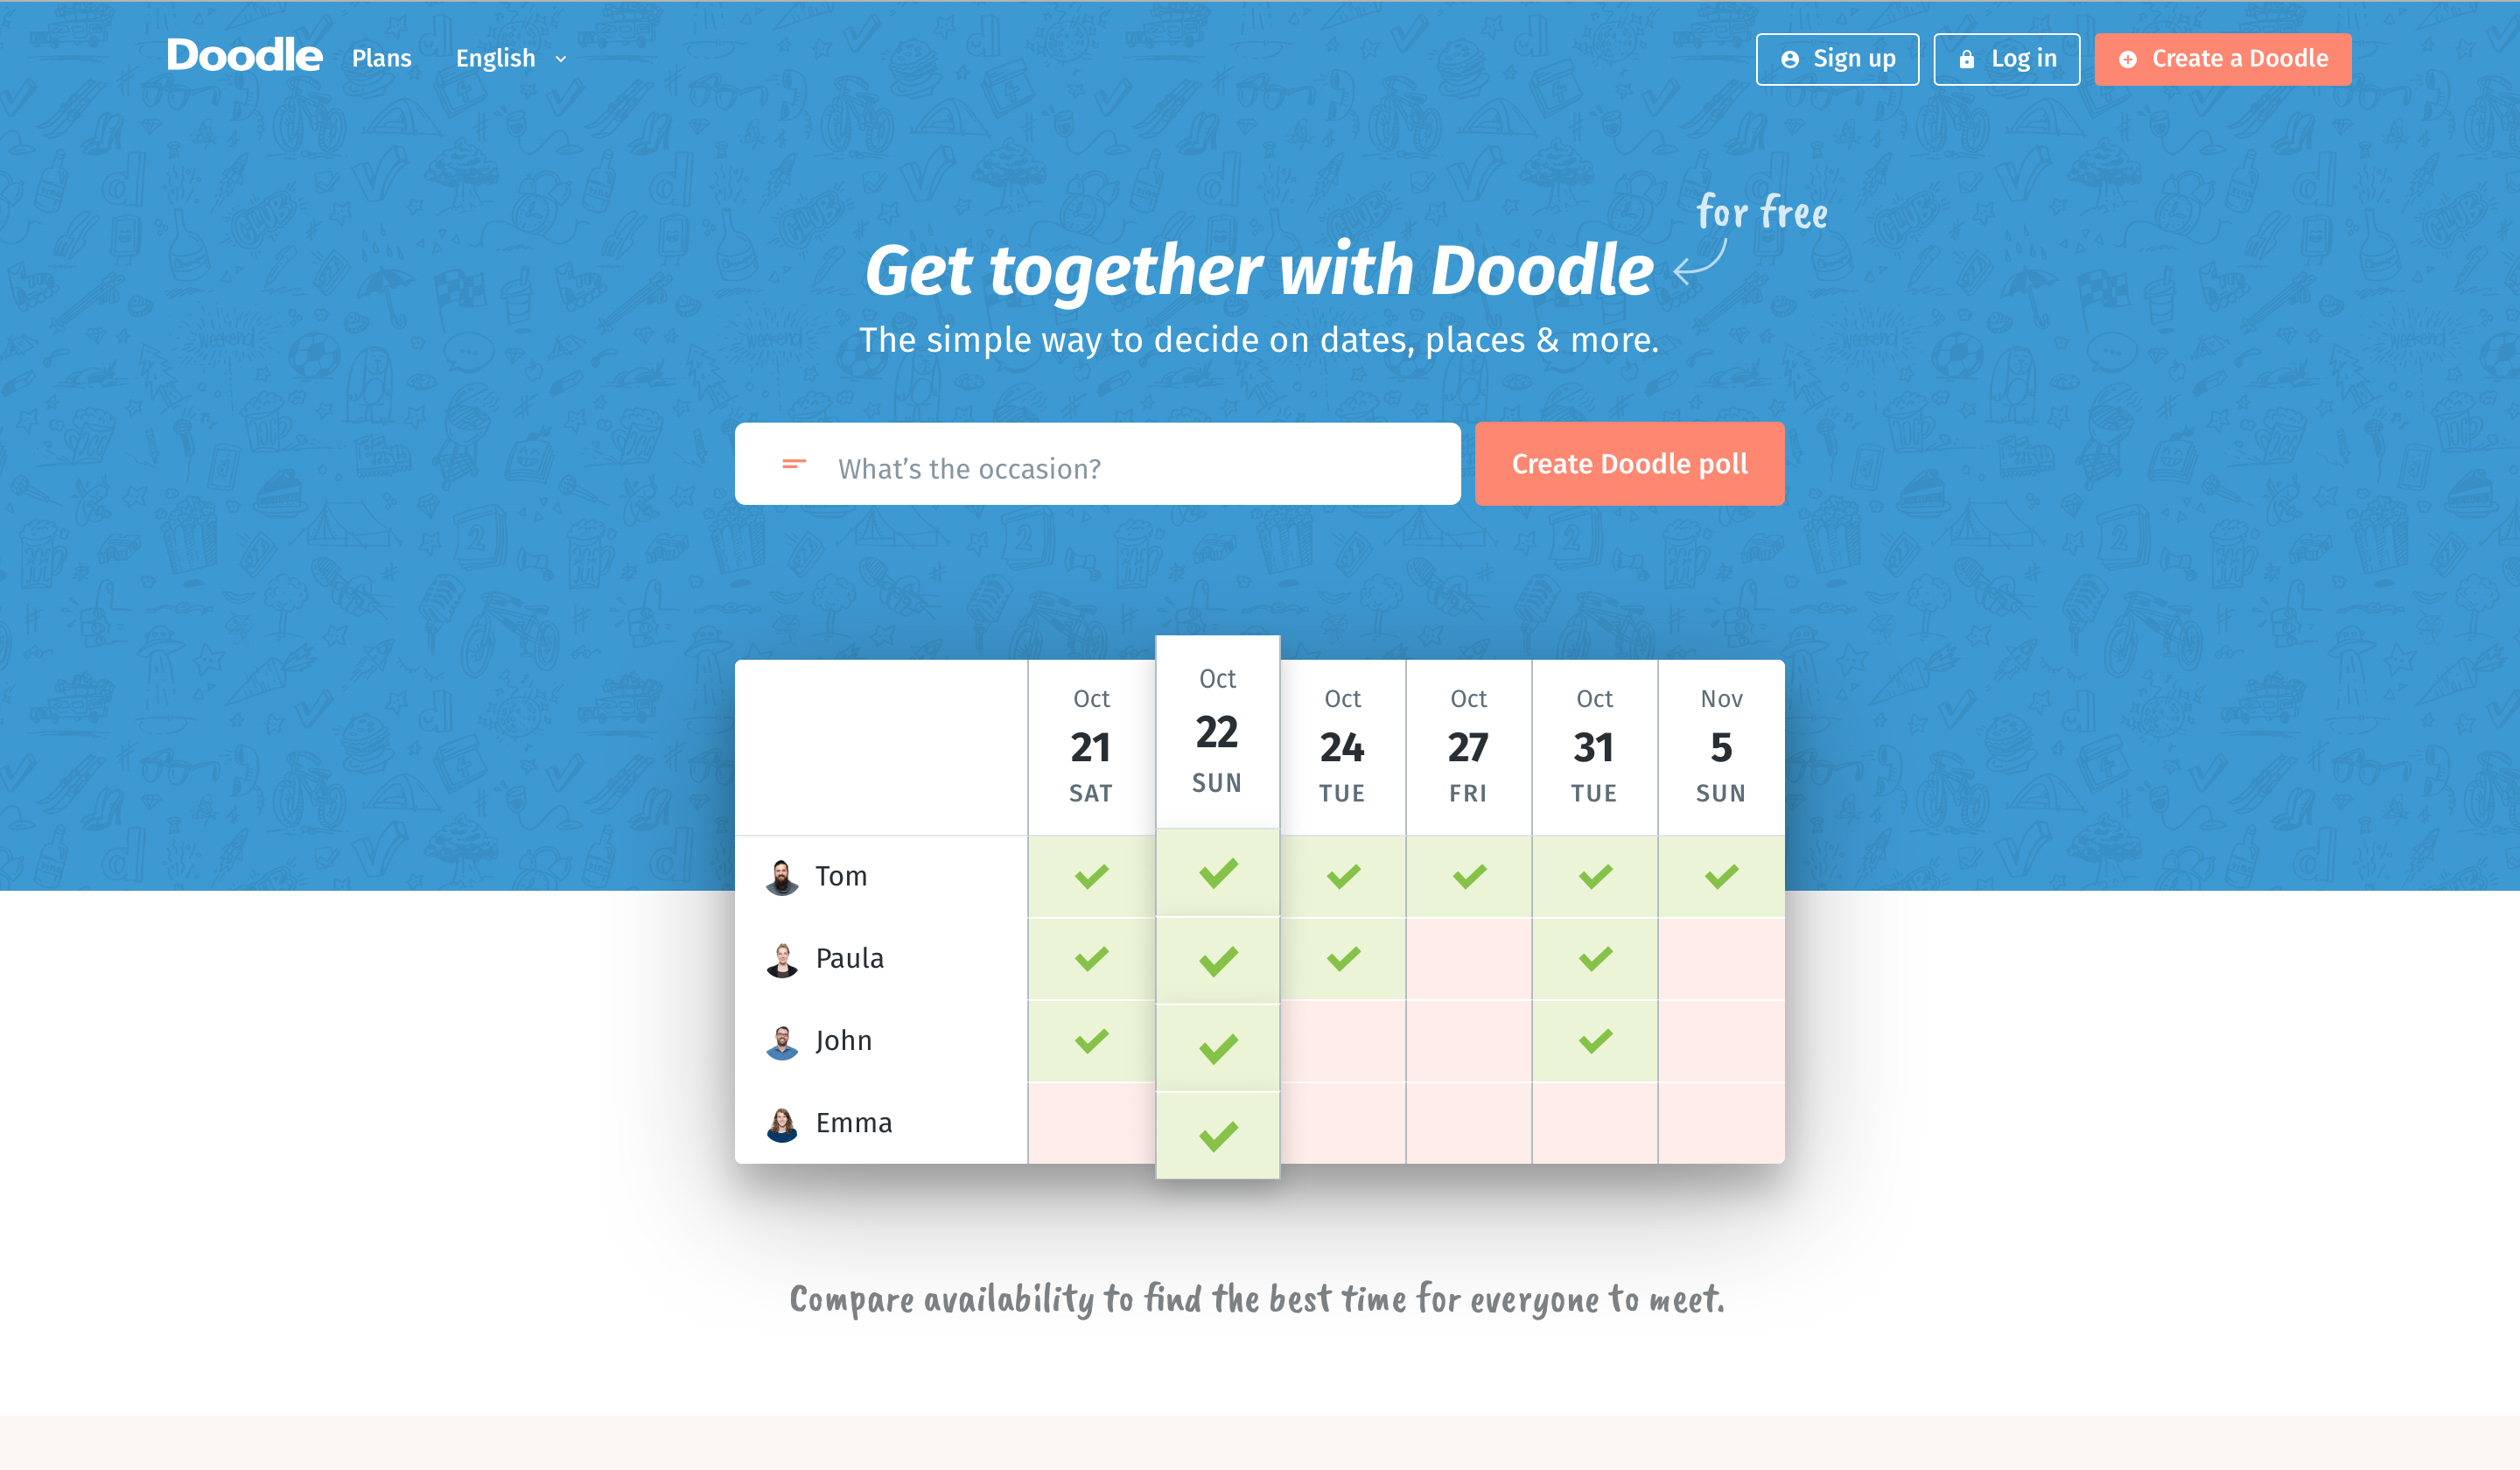
\includegraphics[width=\columnwidth]{{doodle/index.png}}
\label{fig:DOOD_index}
\caption{Doodle homepage}
\end{figure}

\begin{figure}[H]
\centering
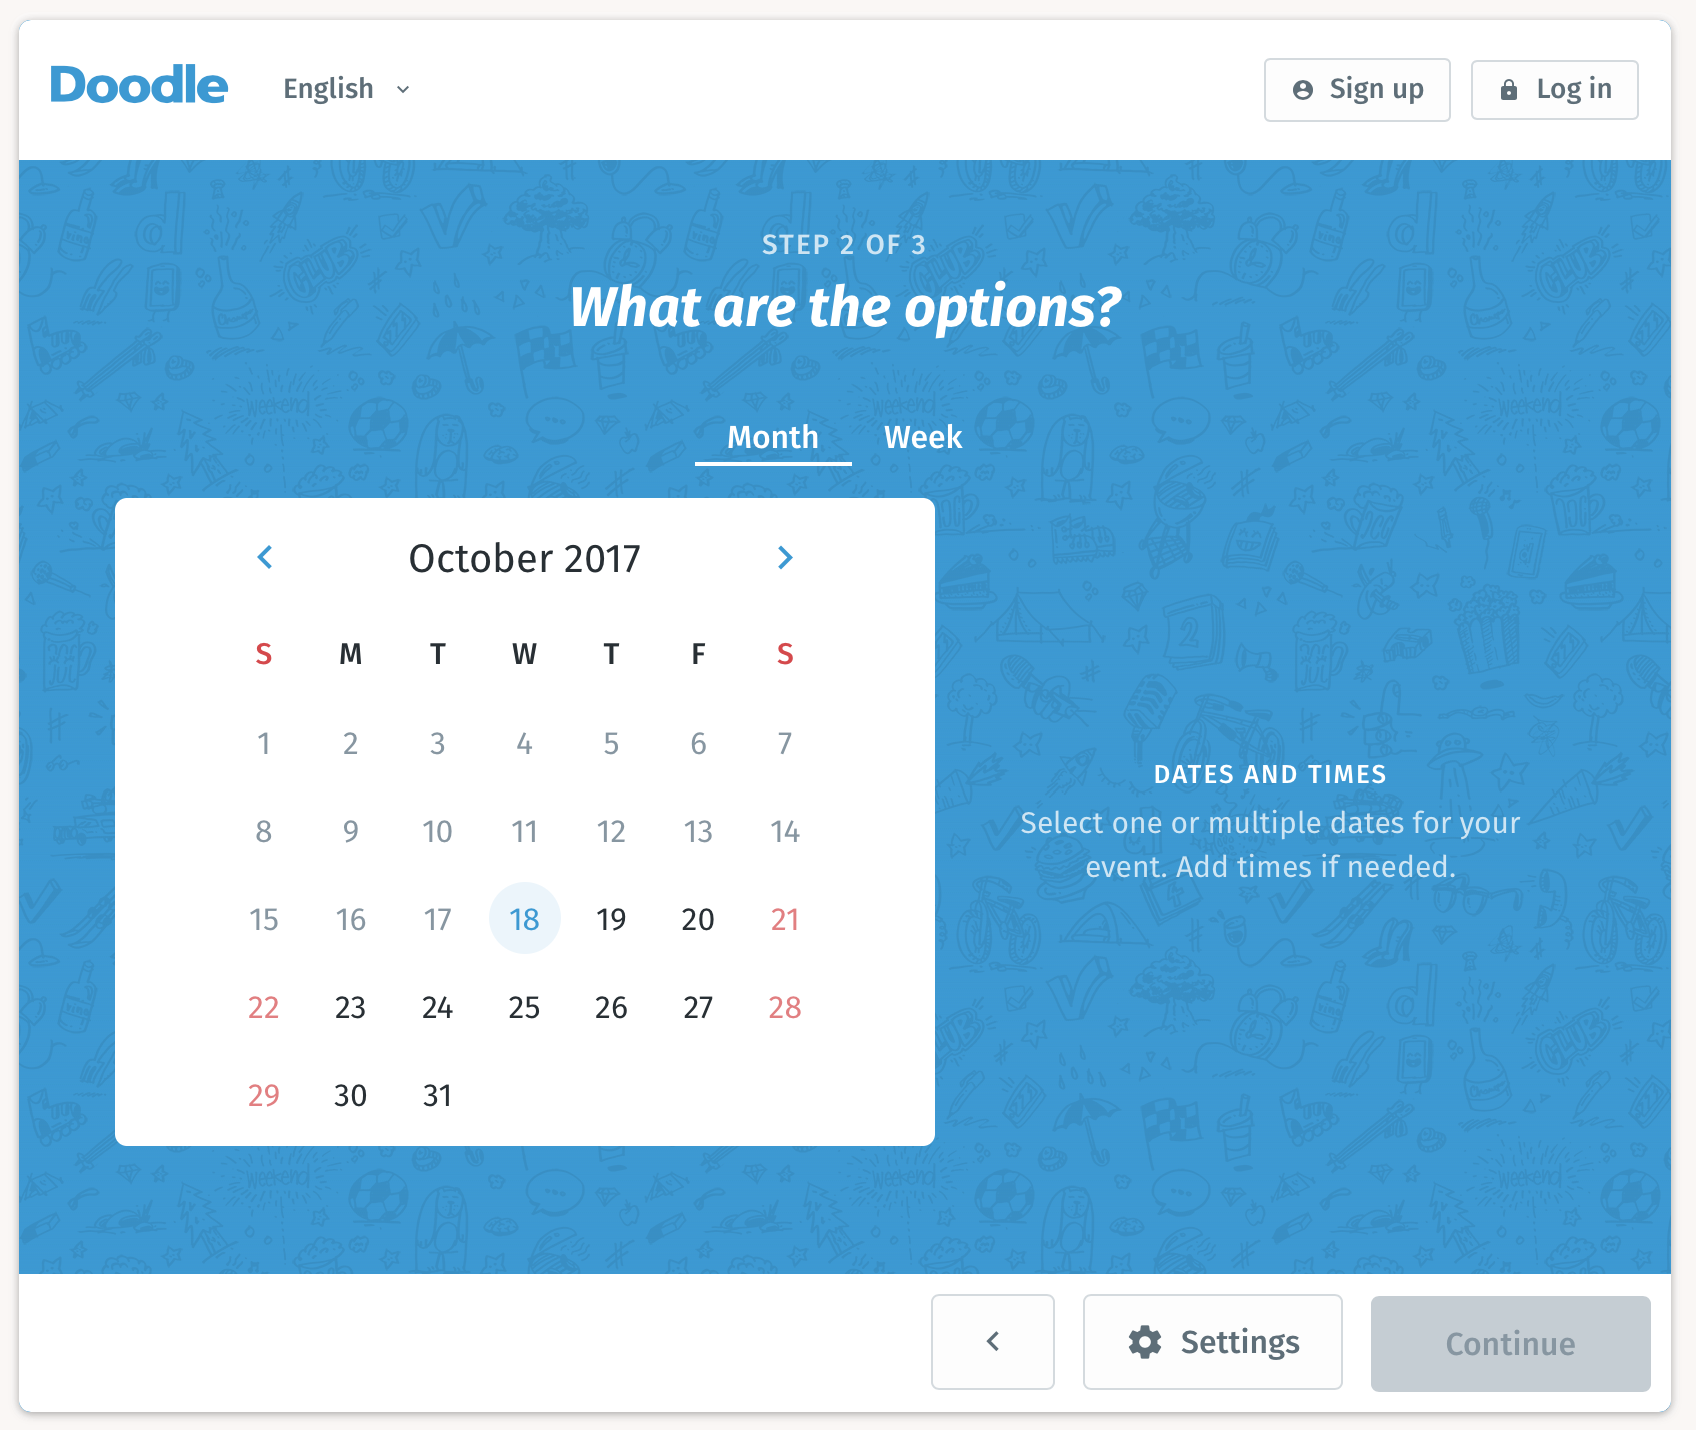
\includegraphics[width=\columnwidth]{{doodle/create-2.png}}
\caption{Create event dialog}
\end{figure}

\begin{figure}[H]
\centering
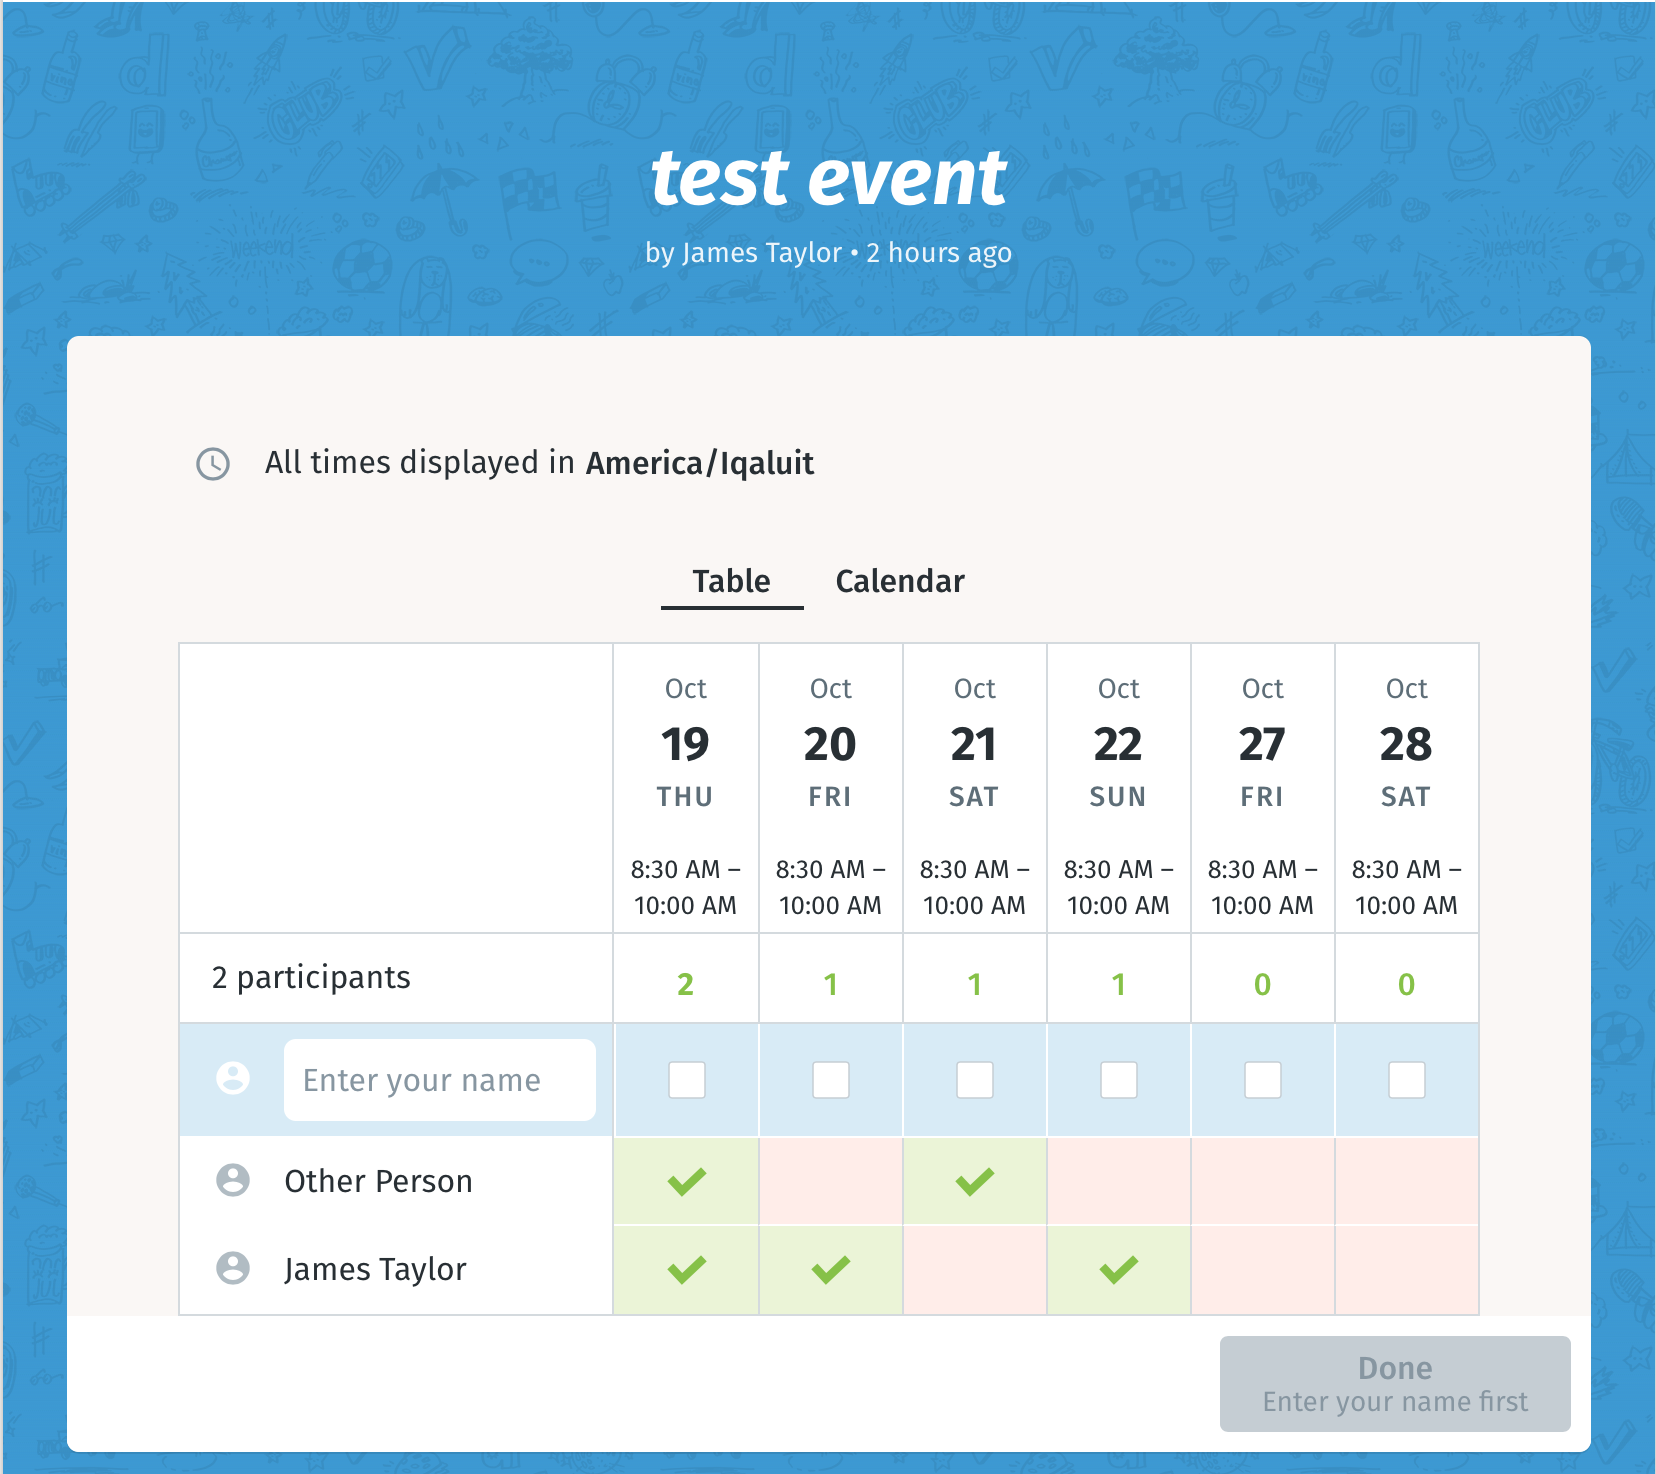
\includegraphics[width=\columnwidth]{{doodle/event.png}}
\caption{Event homepage}
\end{figure}

\begin{figure}[H]
\centering
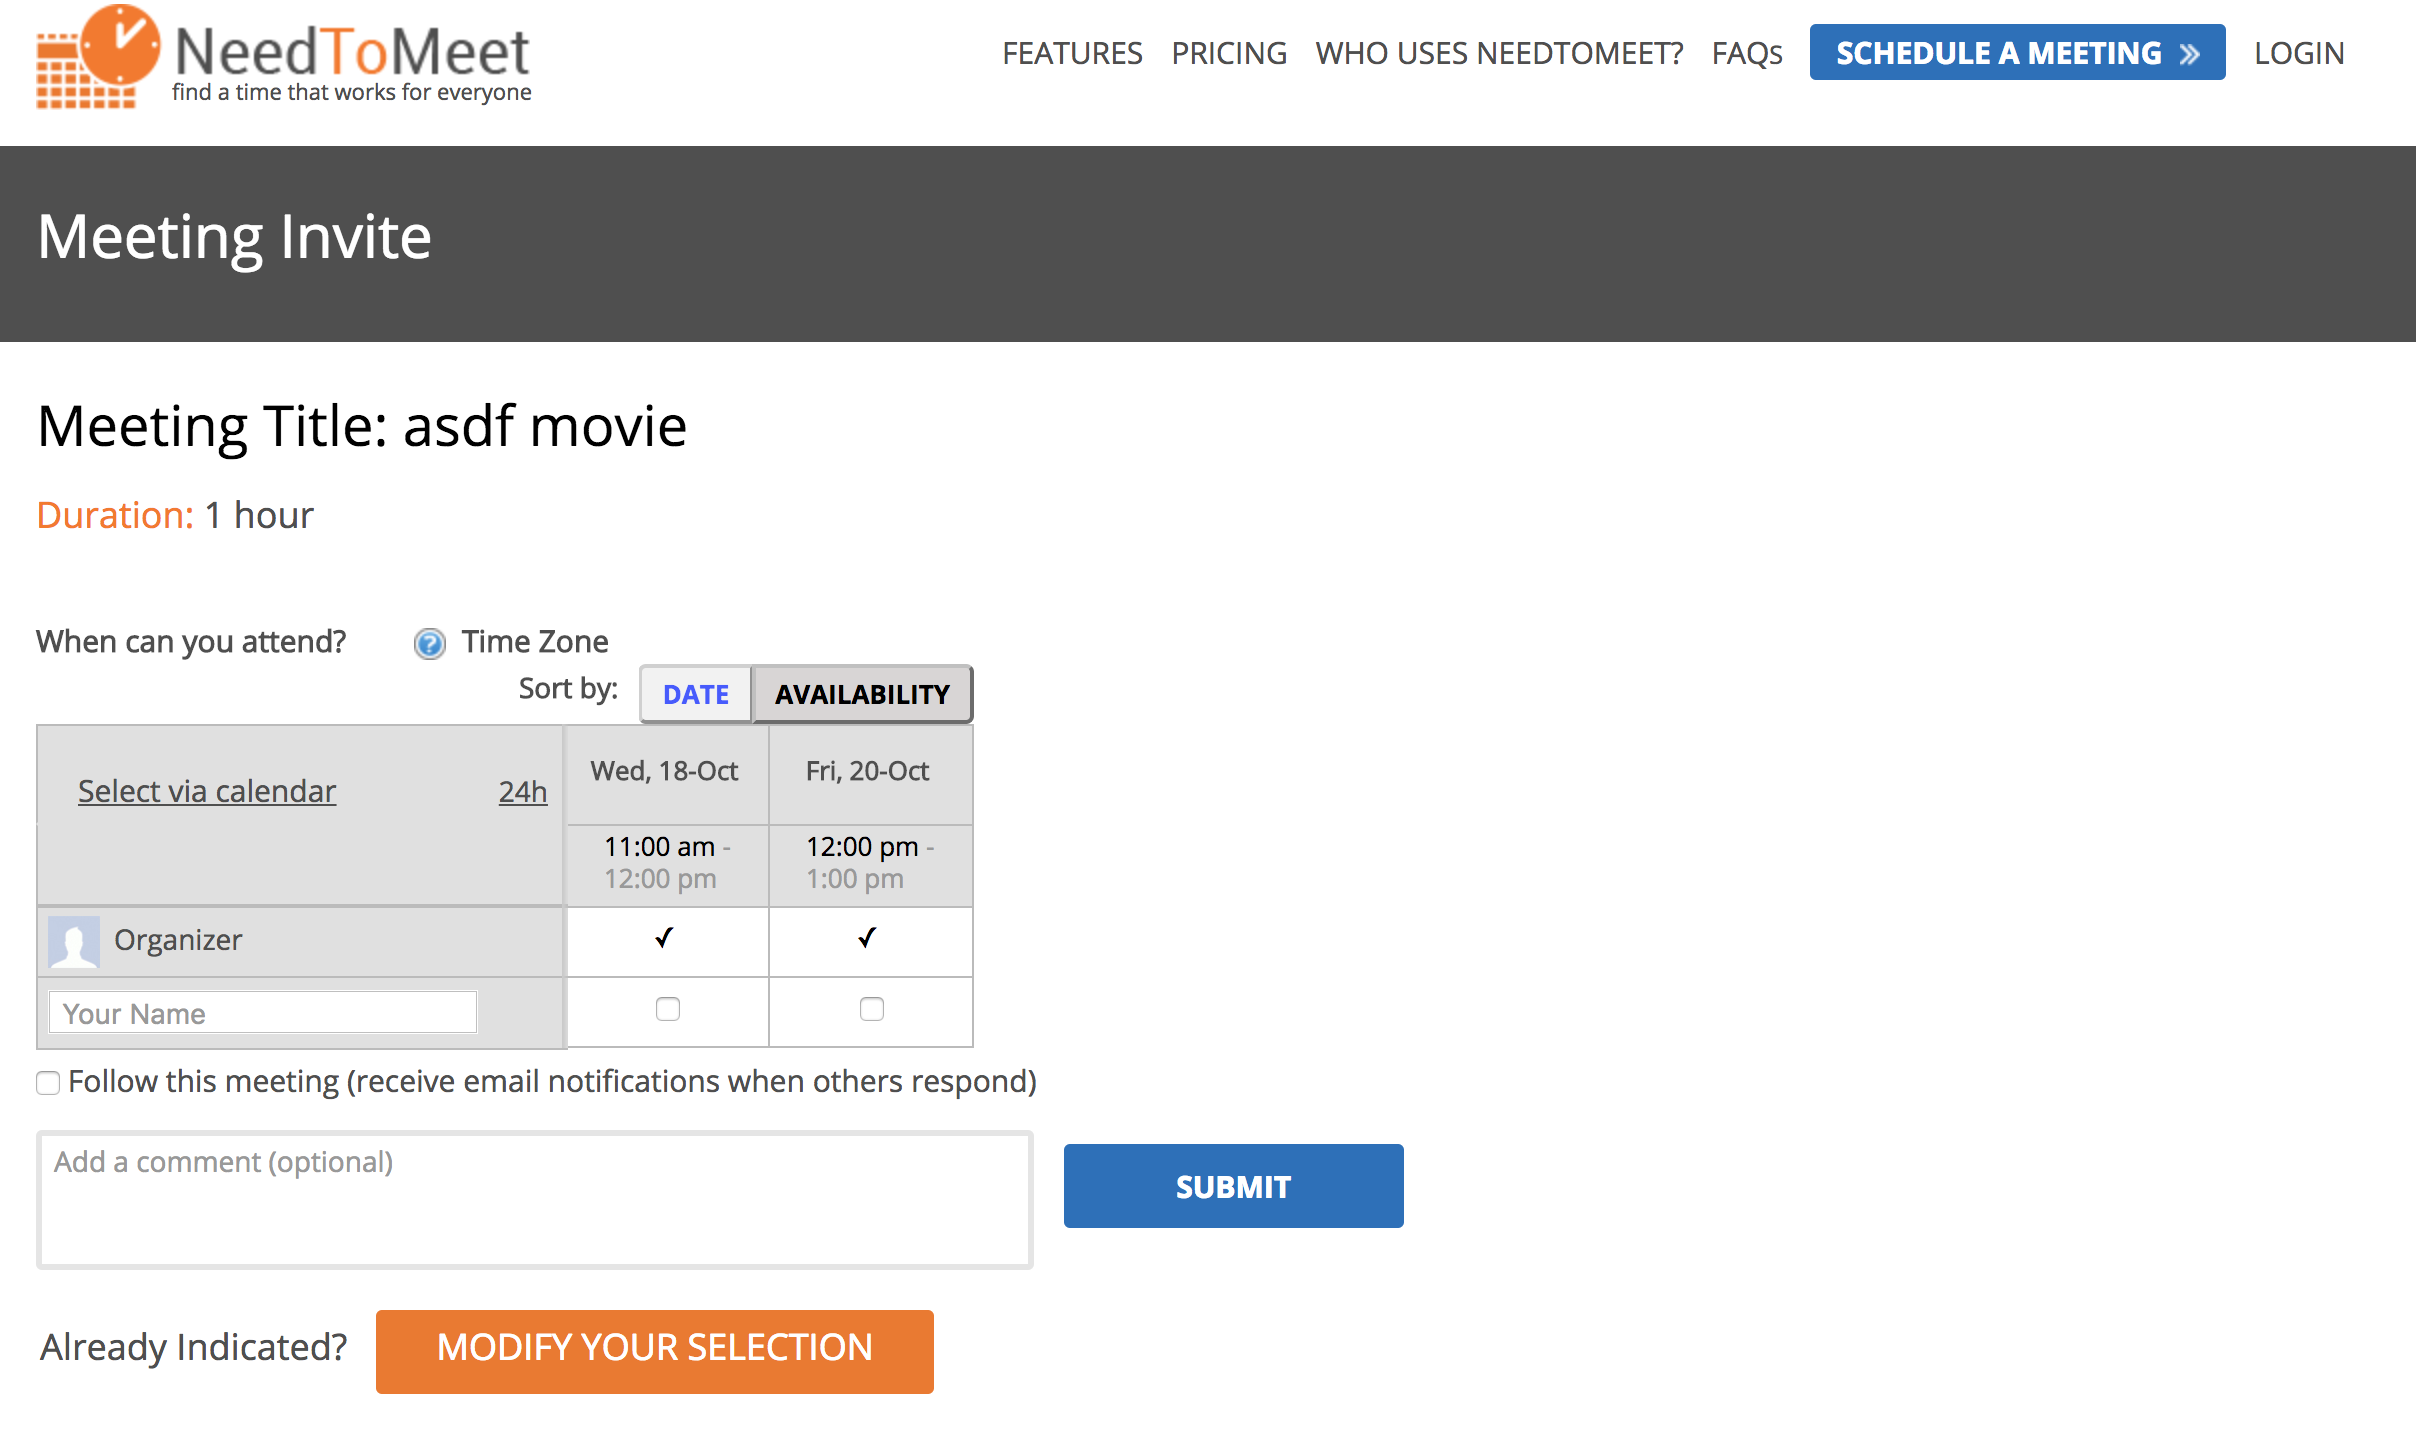
\includegraphics[width=\columnwidth]{{figures/NeedToMeet/Creator_Images/1.png}}
\caption{Need To Meet Homepage}
\end{figure}
%%%%%%

\begin{figure}[H]
\centering
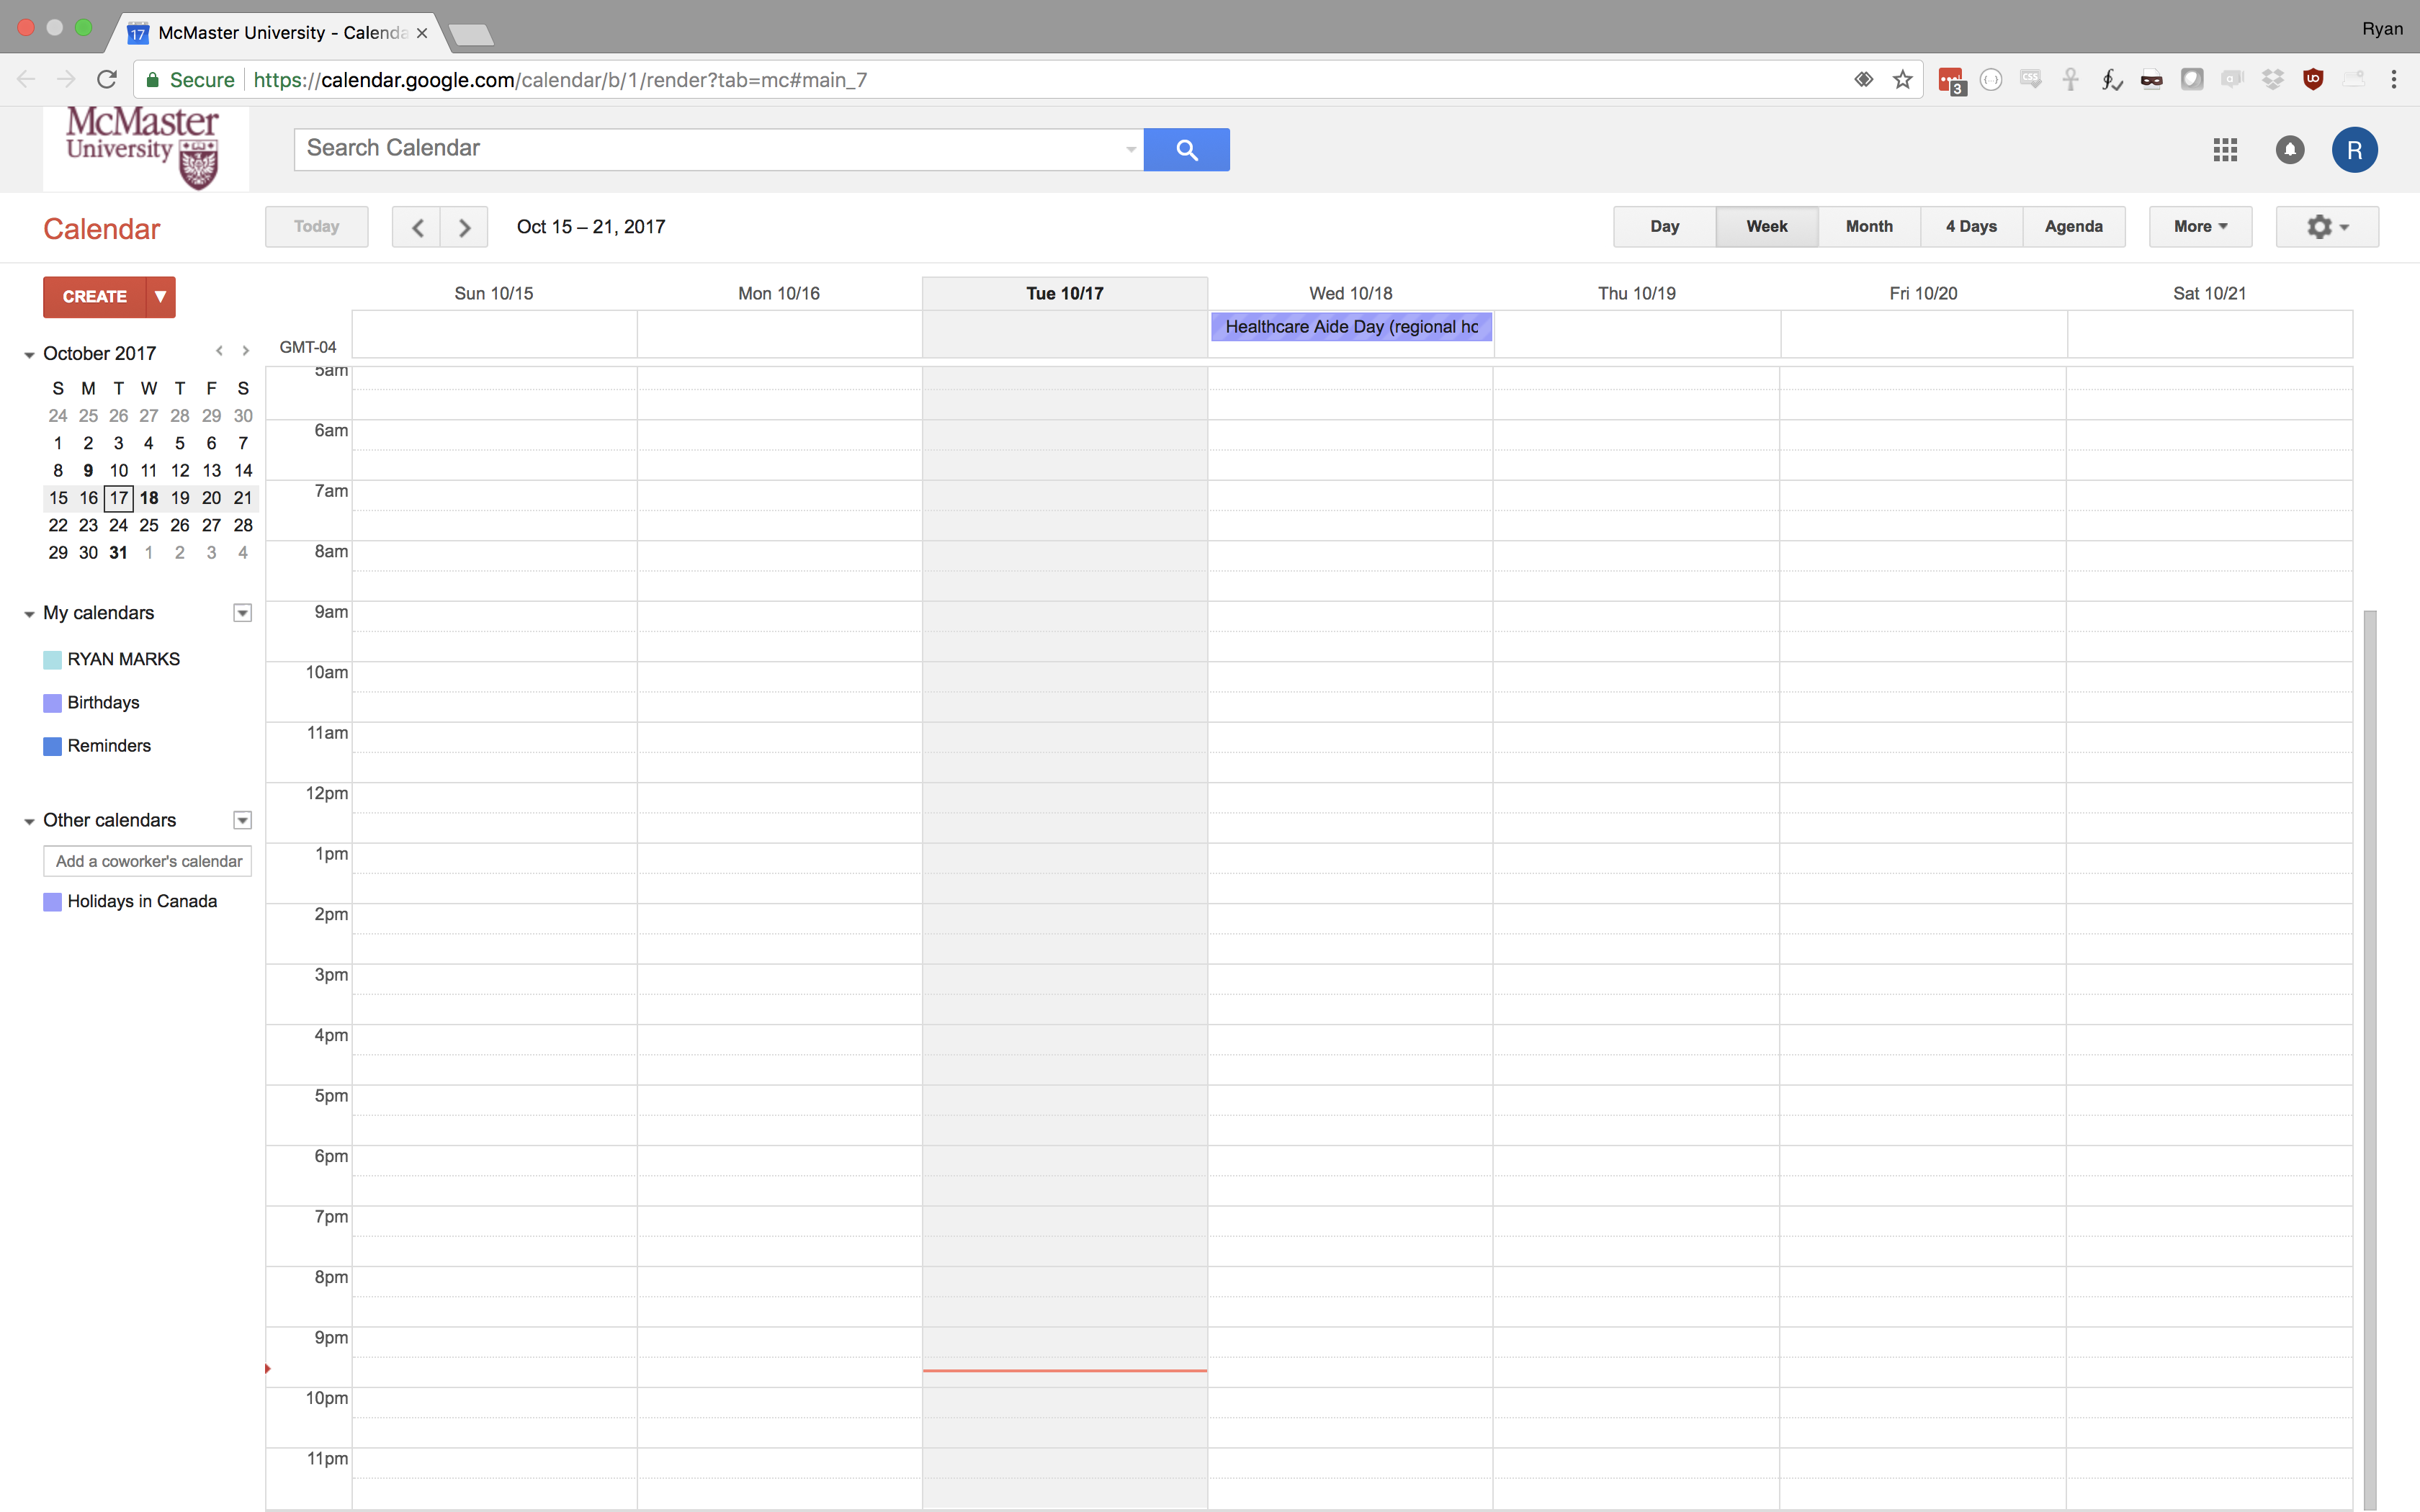
\includegraphics[width=\columnwidth]{{google/Invite1.1}}
\caption{Subtask 1.1 of the invitation procedure for Google Calendar}
\end{figure}

\begin{figure}[H]
\centering
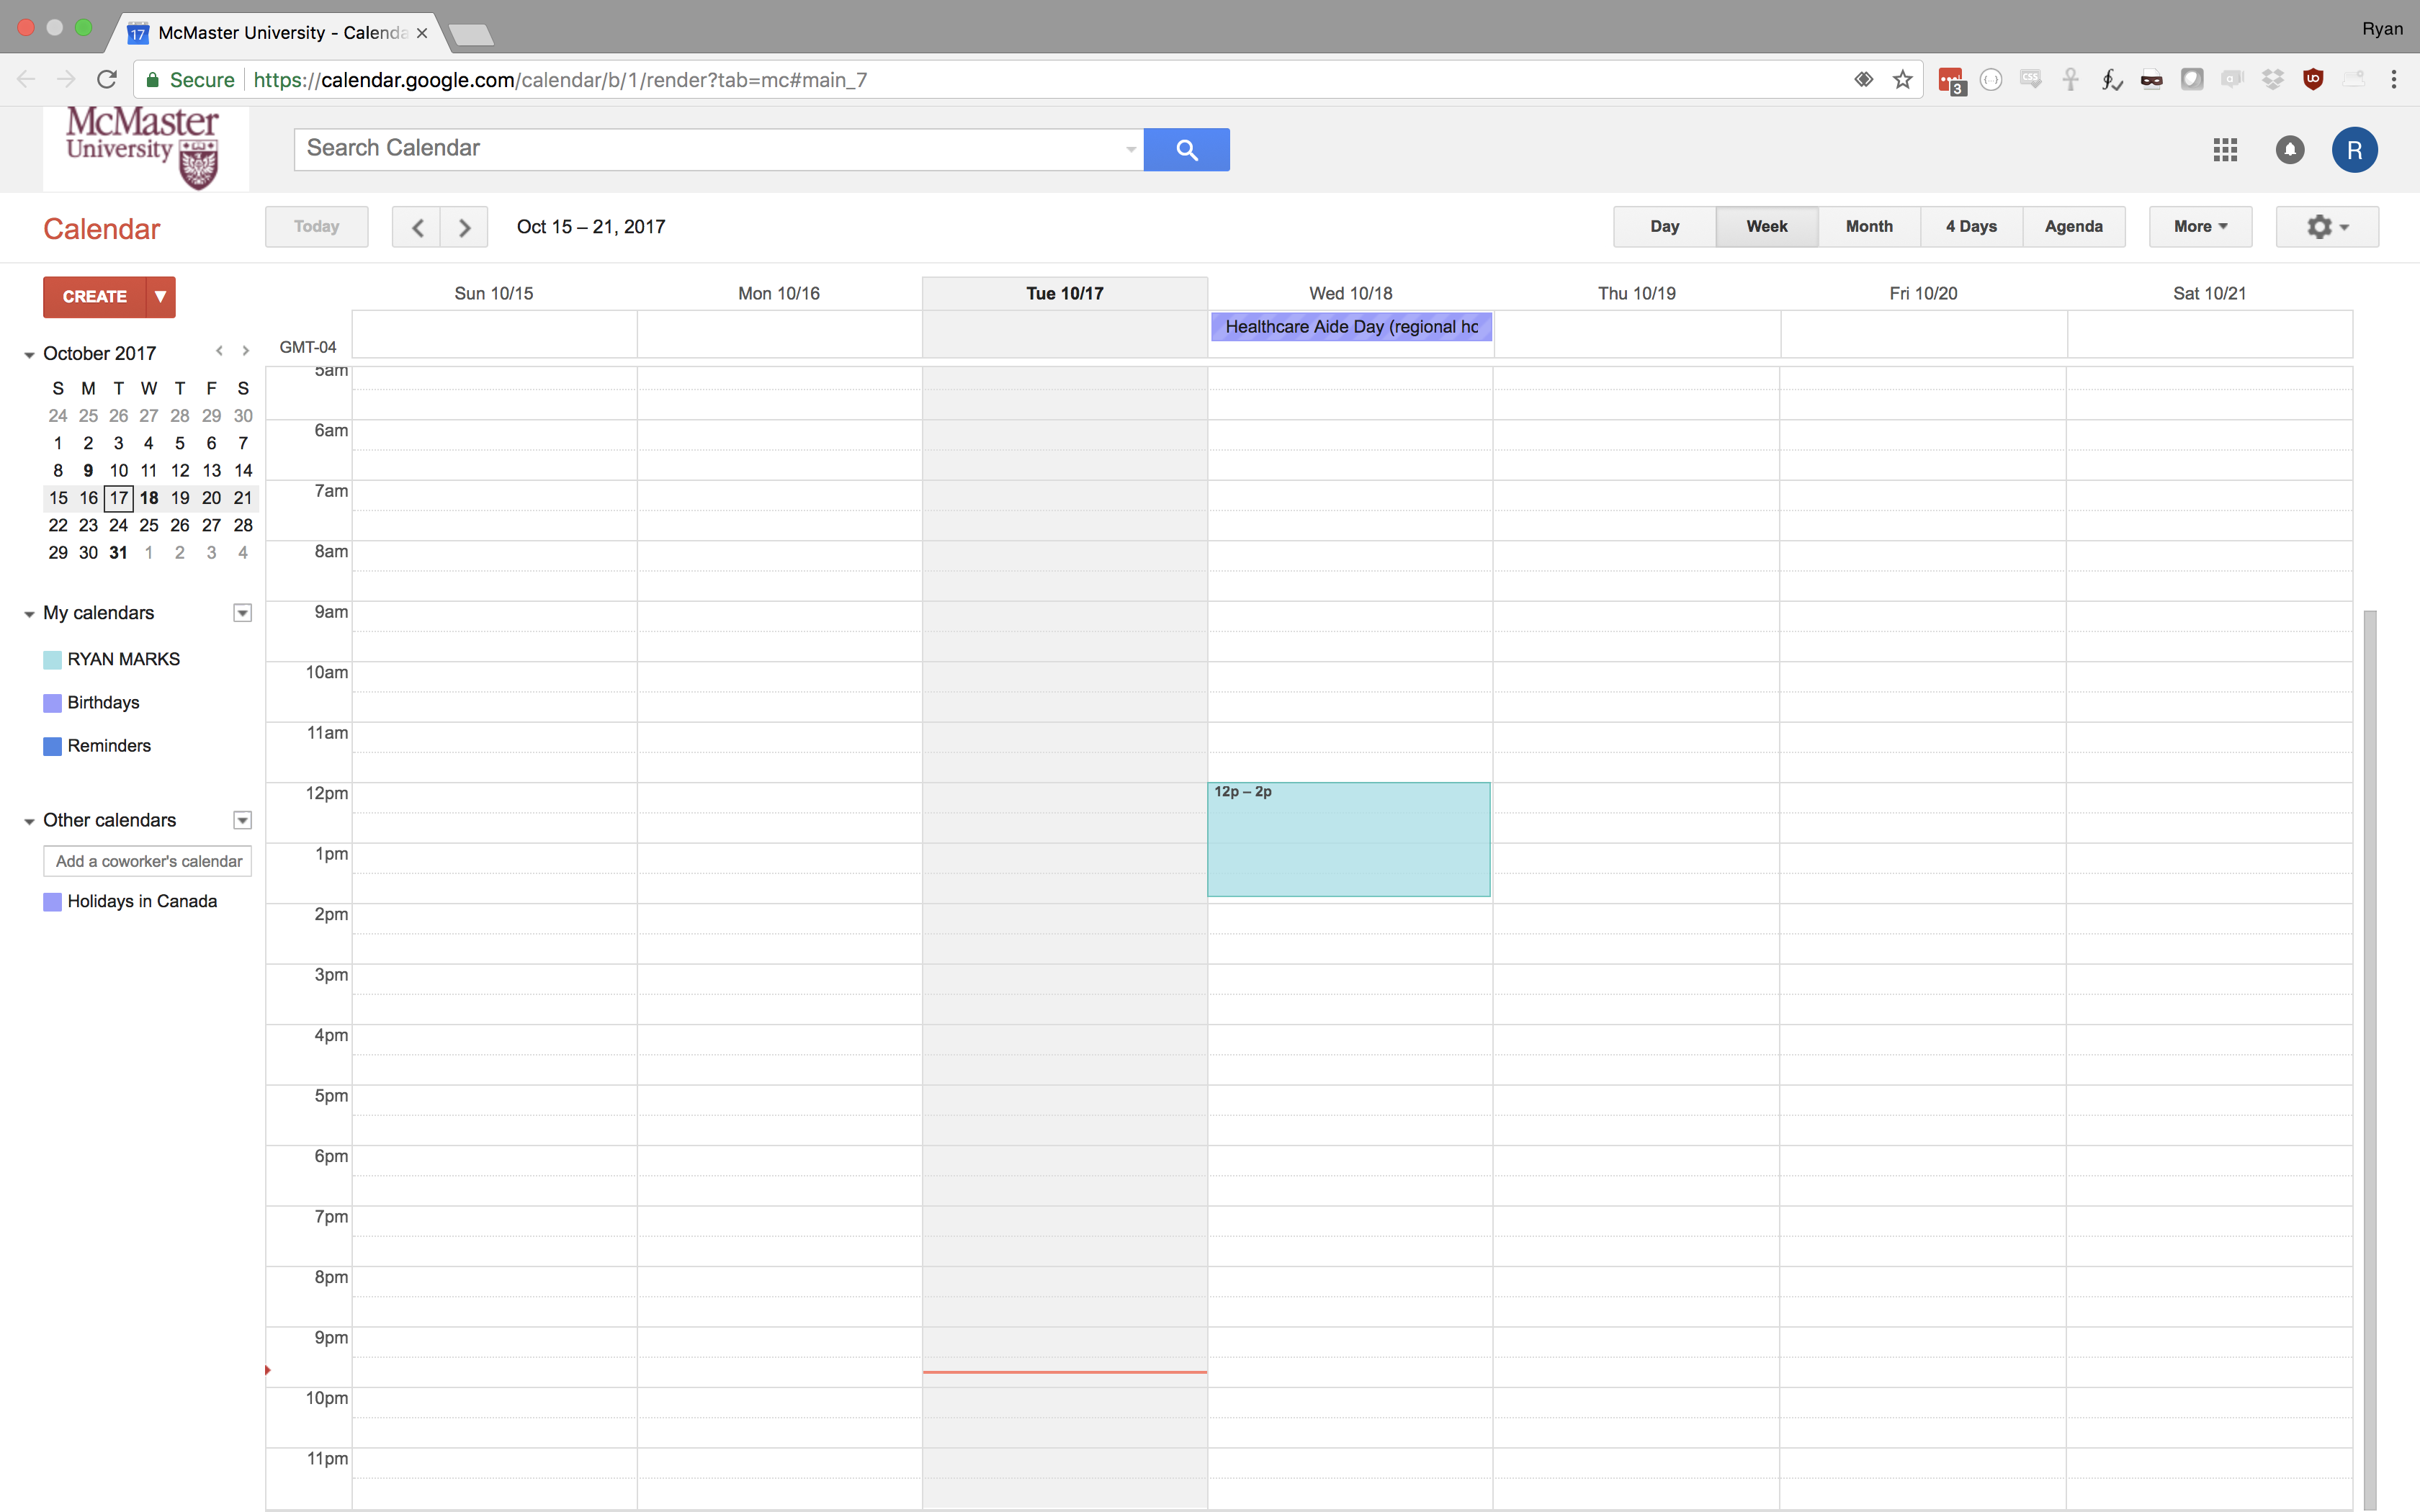
\includegraphics[width=\columnwidth]{{google/Invite1.2}}
\caption{Subtask 1.2 of the invitation procedure for Google Calendar}
\end{figure}

\begin{figure}[H]
\centering
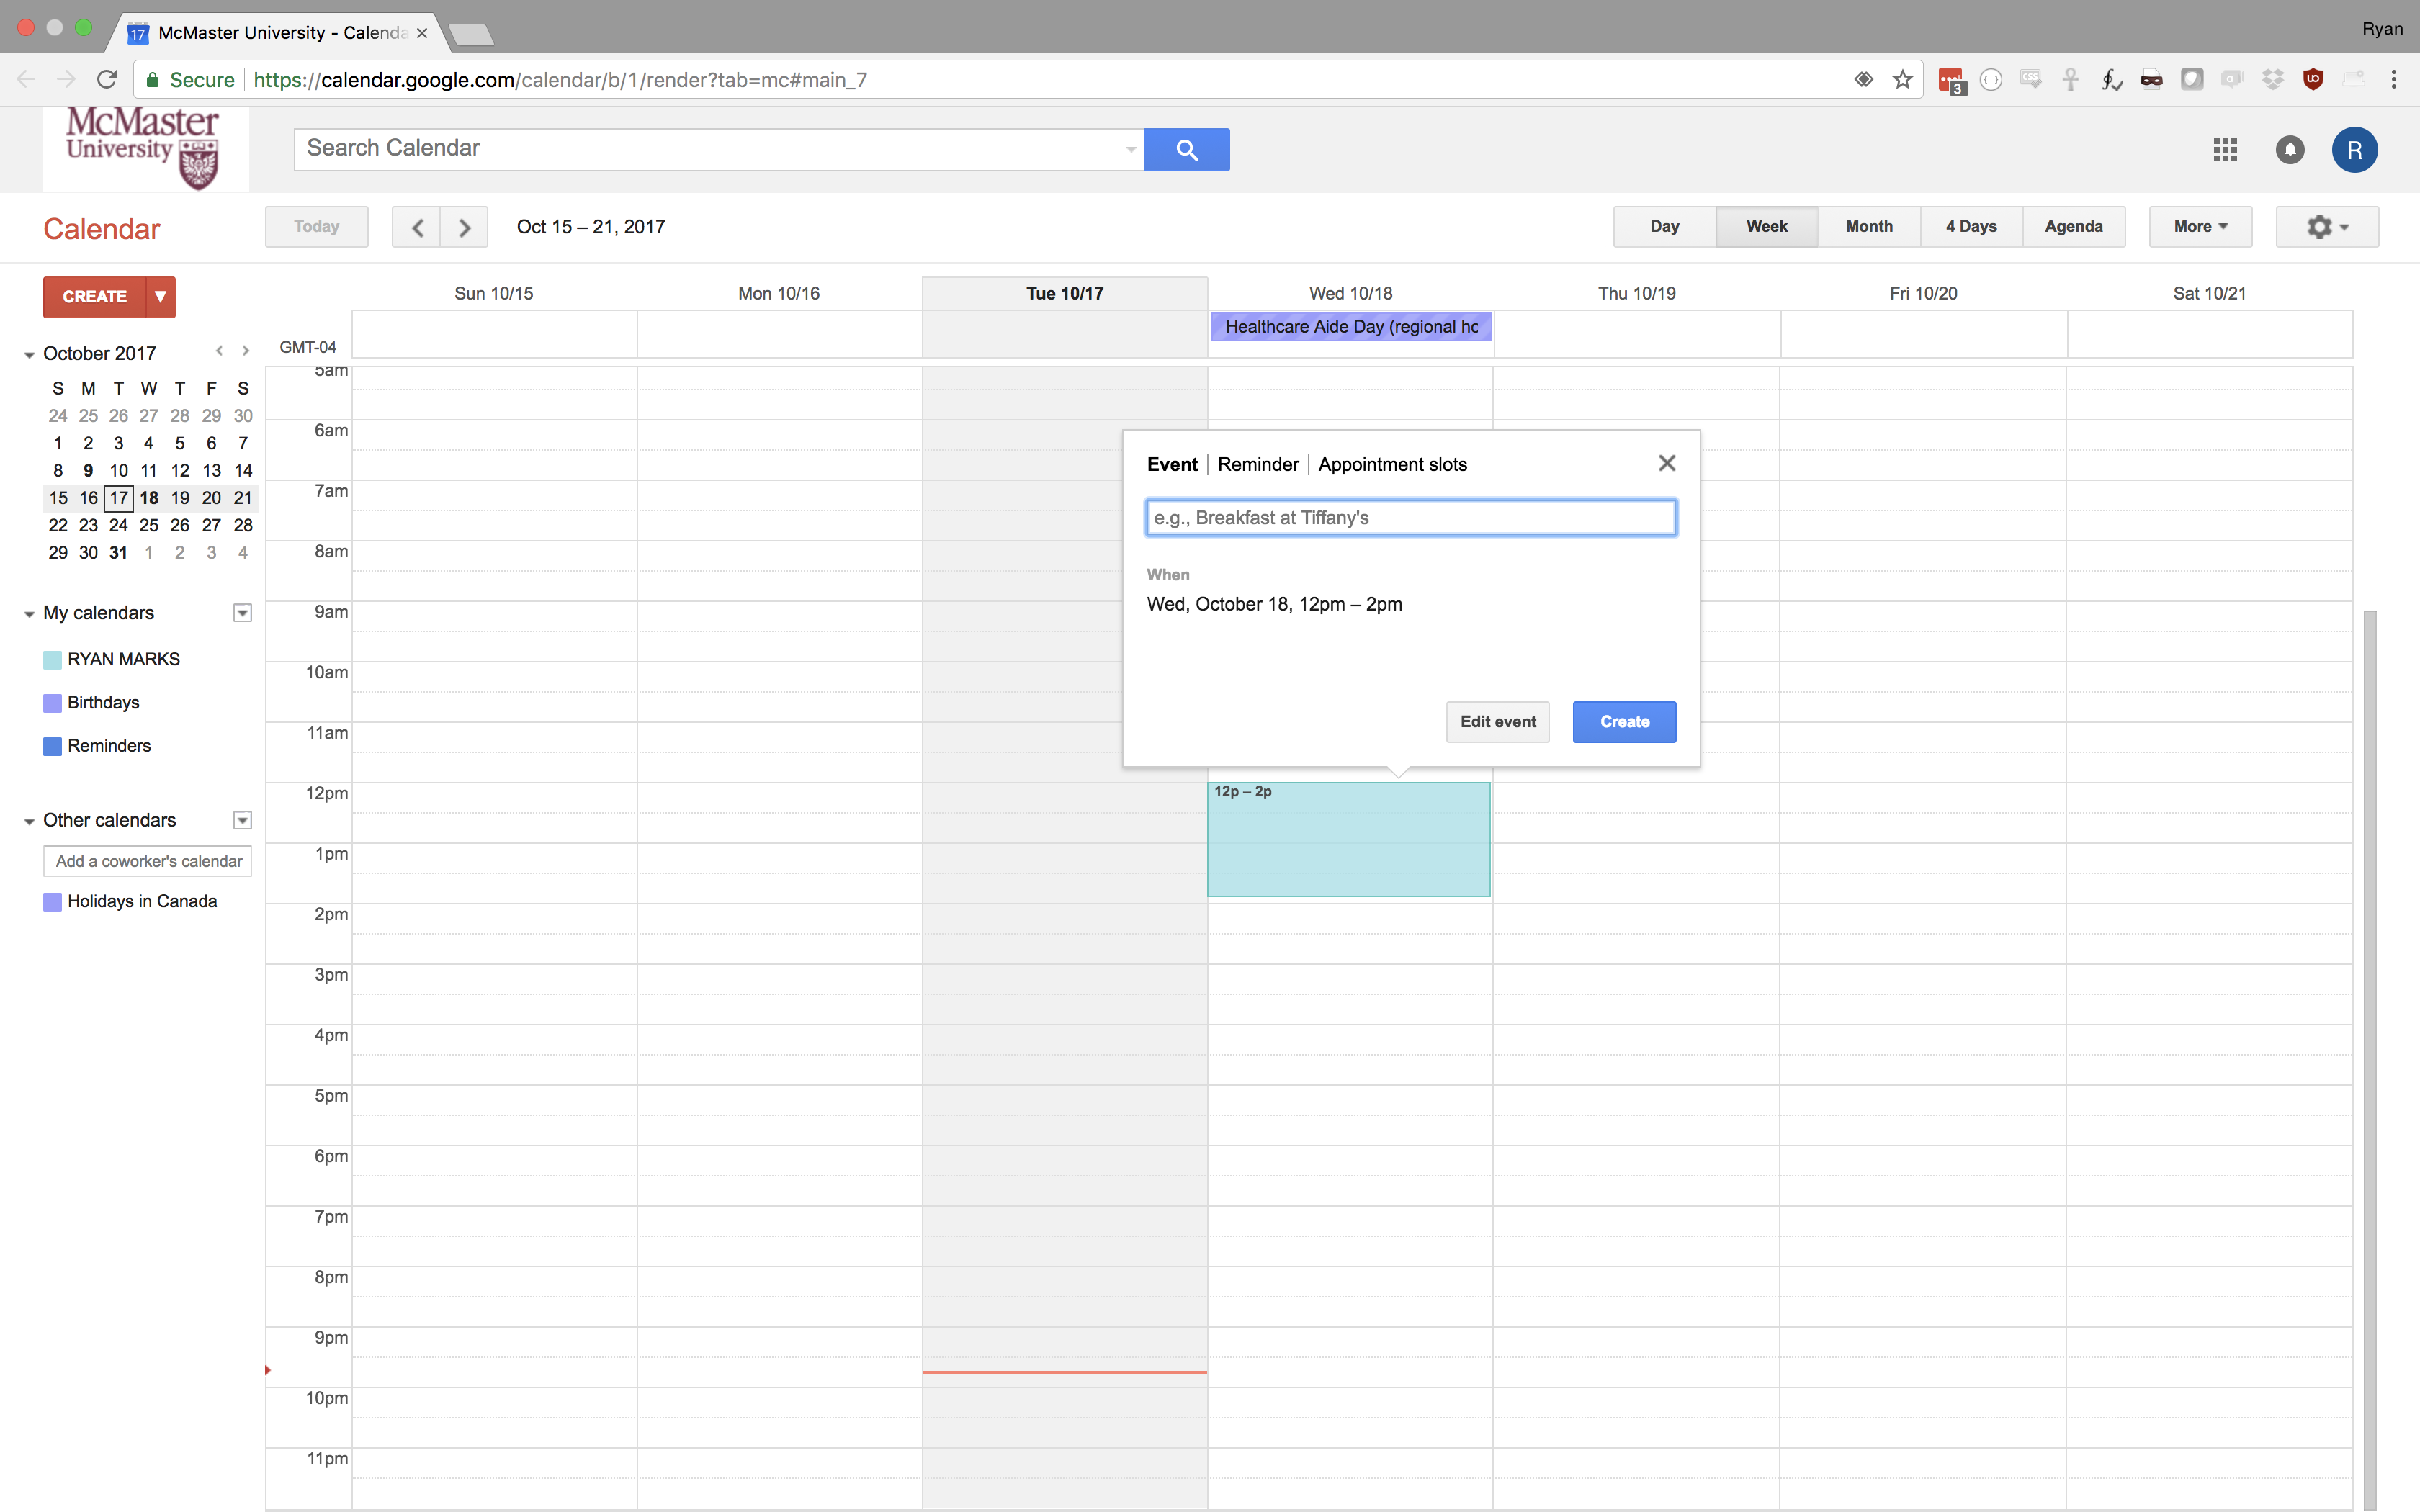
\includegraphics[width=\columnwidth]{{google/Invite1.3}}
\caption{Befort subtask 1.3 of the invitation procedure for Google Calendar}
\end{figure}

\begin{figure}[H]
\centering
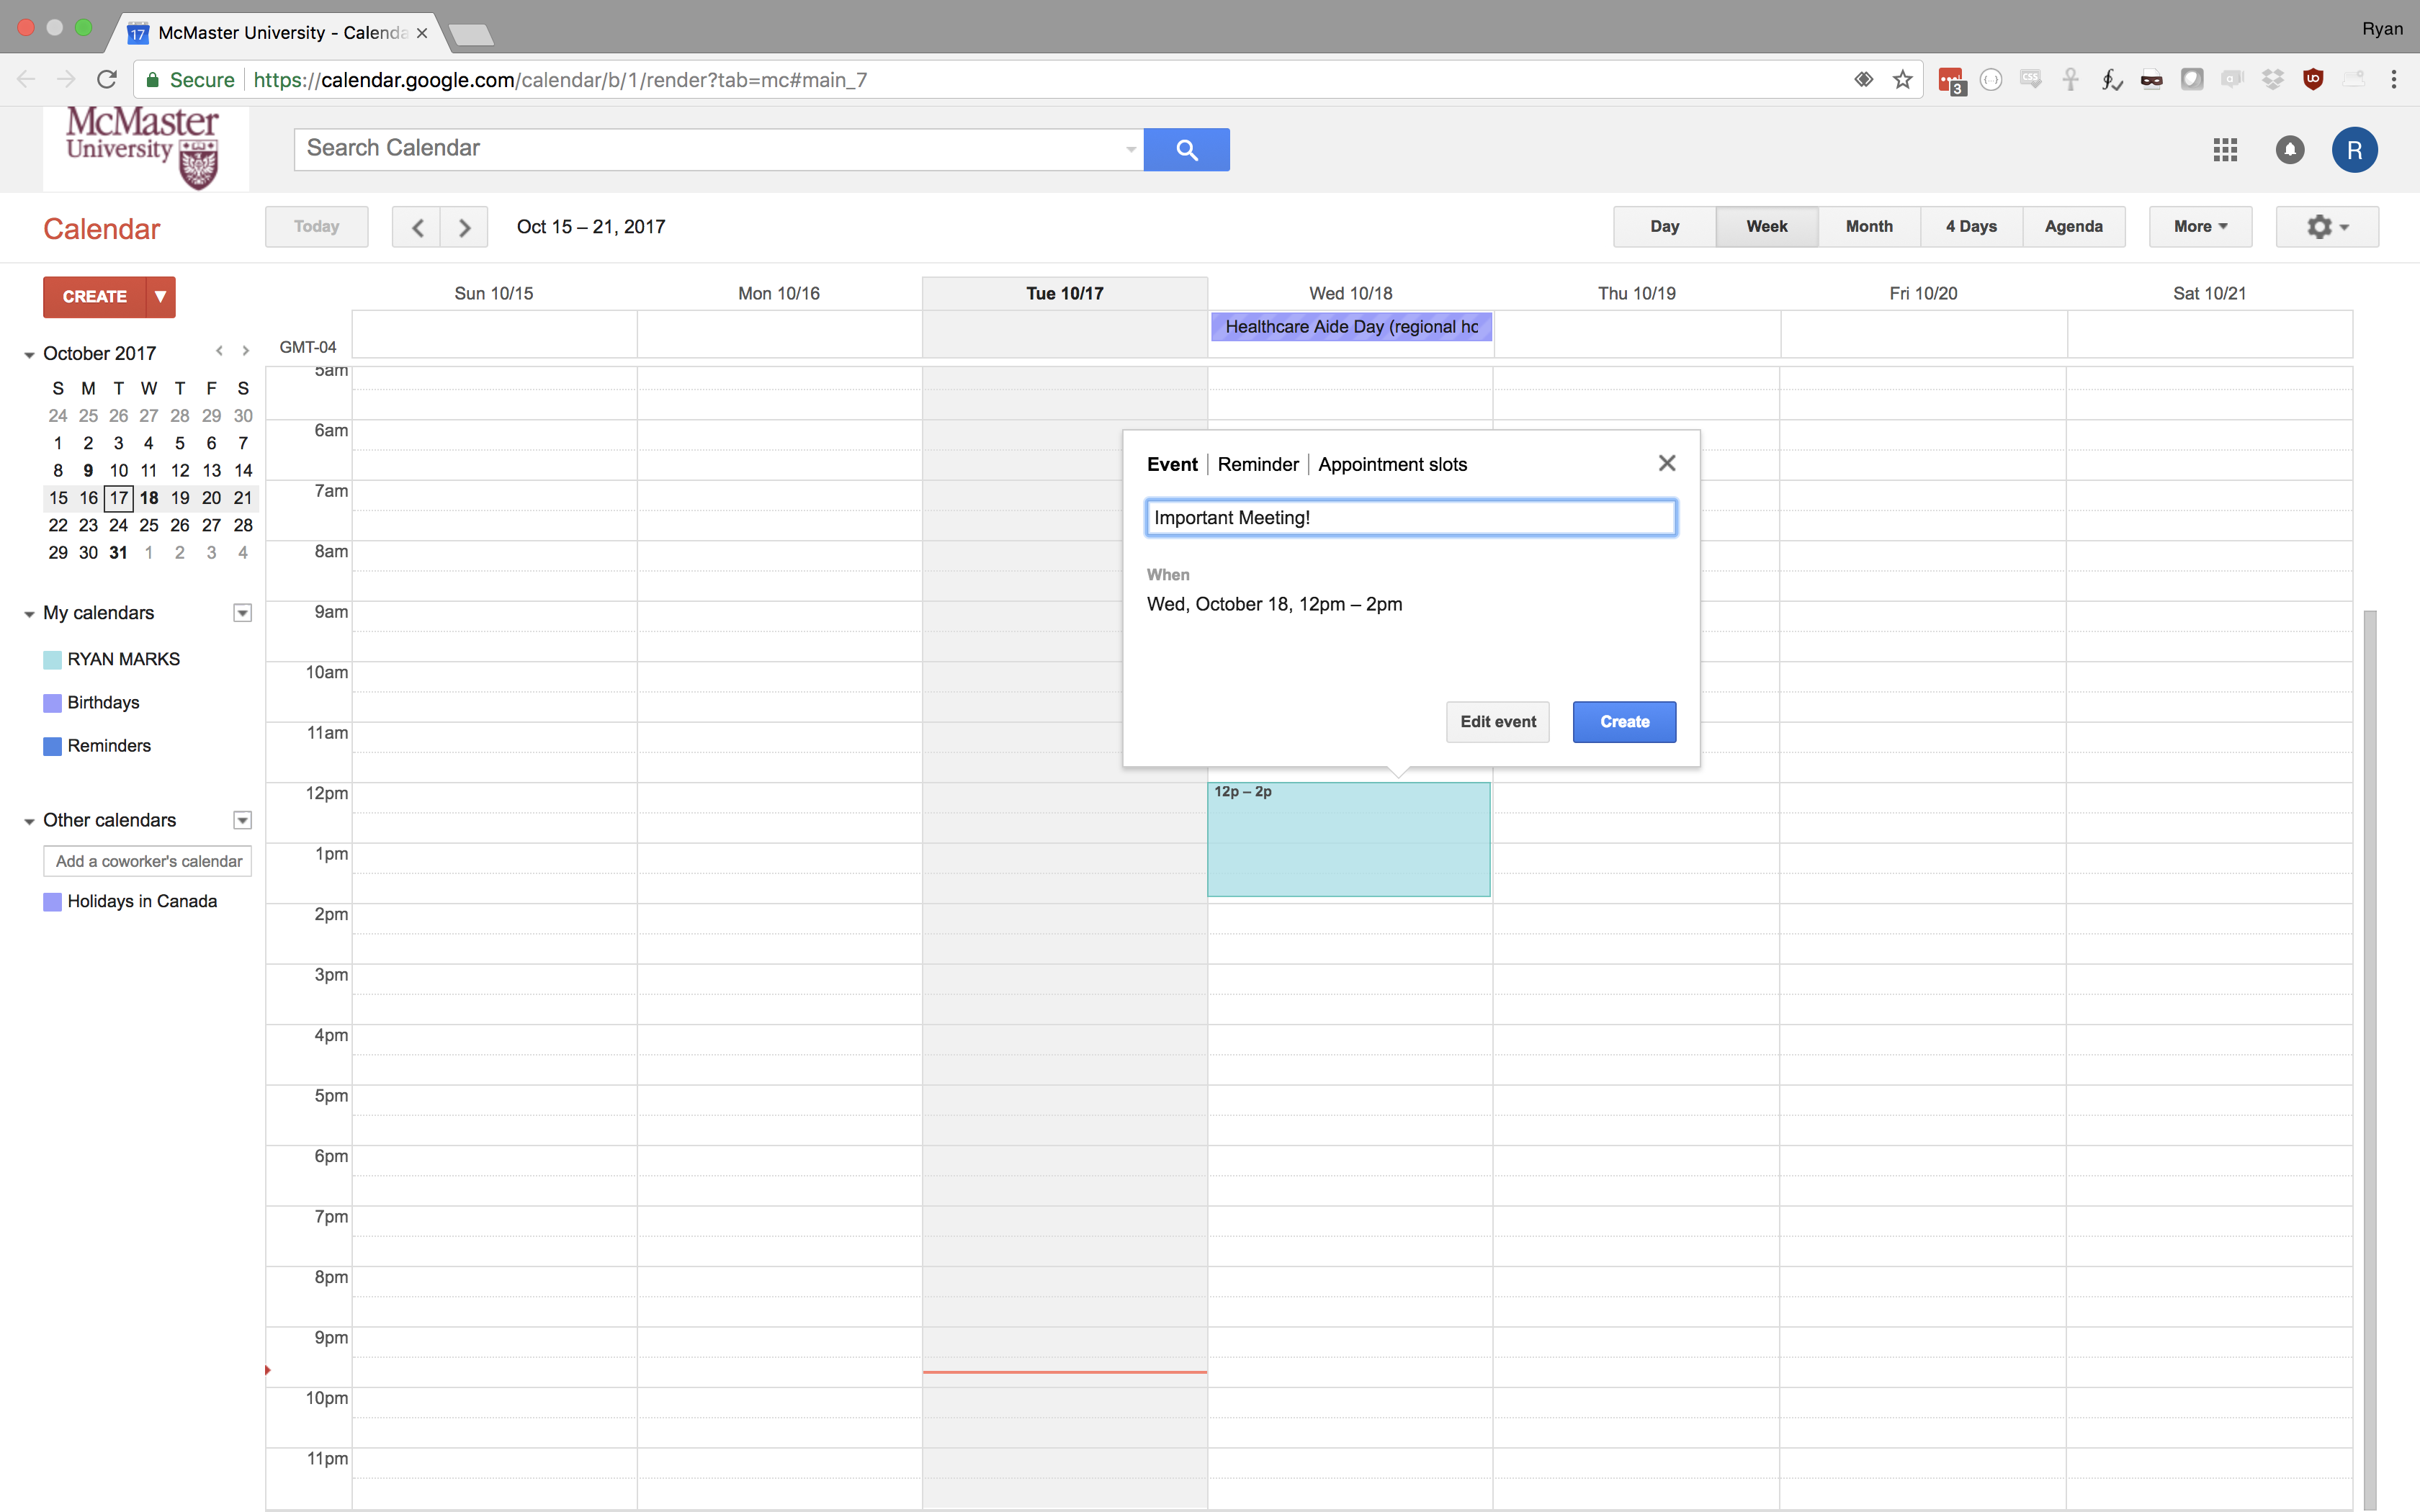
\includegraphics[width=\columnwidth]{{google/Invite1.3end}}
\caption{After subtask 1.3 of the invitation procedure for Google Calendar}
\end{figure}

\begin{figure}[H]
\centering
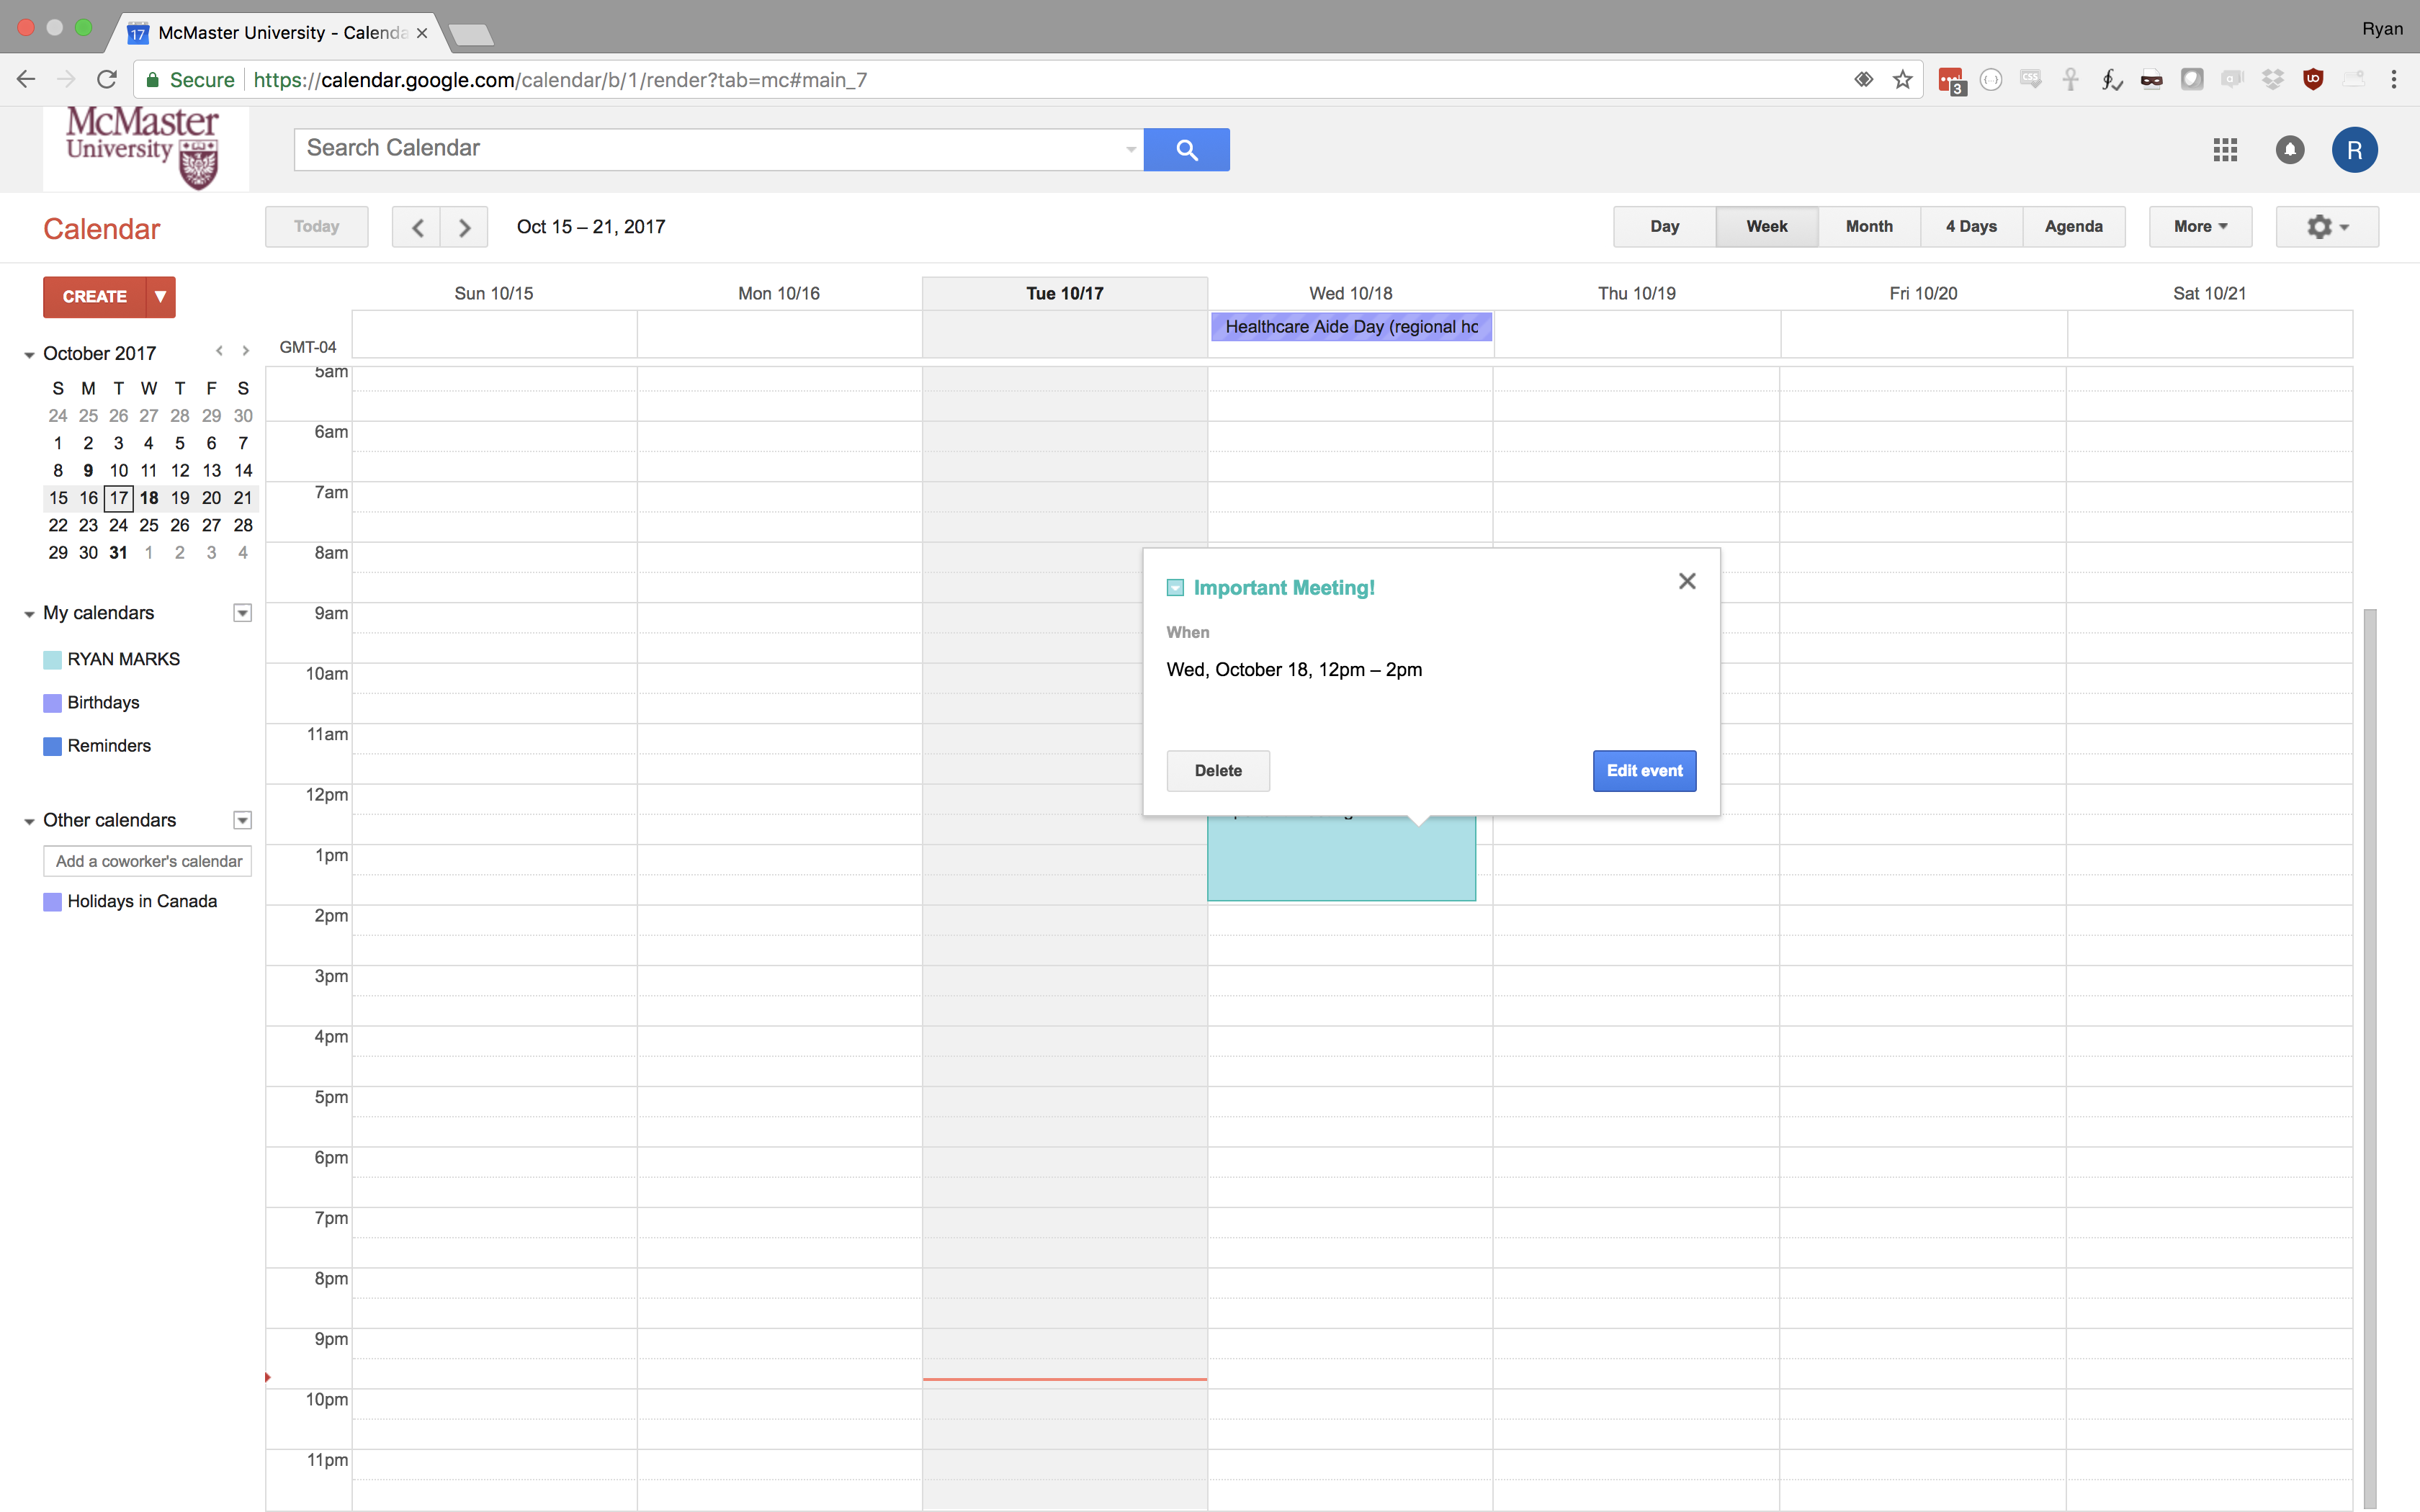
\includegraphics[width=\columnwidth]{{google/Invite2.1}}
\caption{Before subtask 2.1 of the invitation procedure for Google Calendar}
\end{figure}

\begin{figure}[H]
\centering
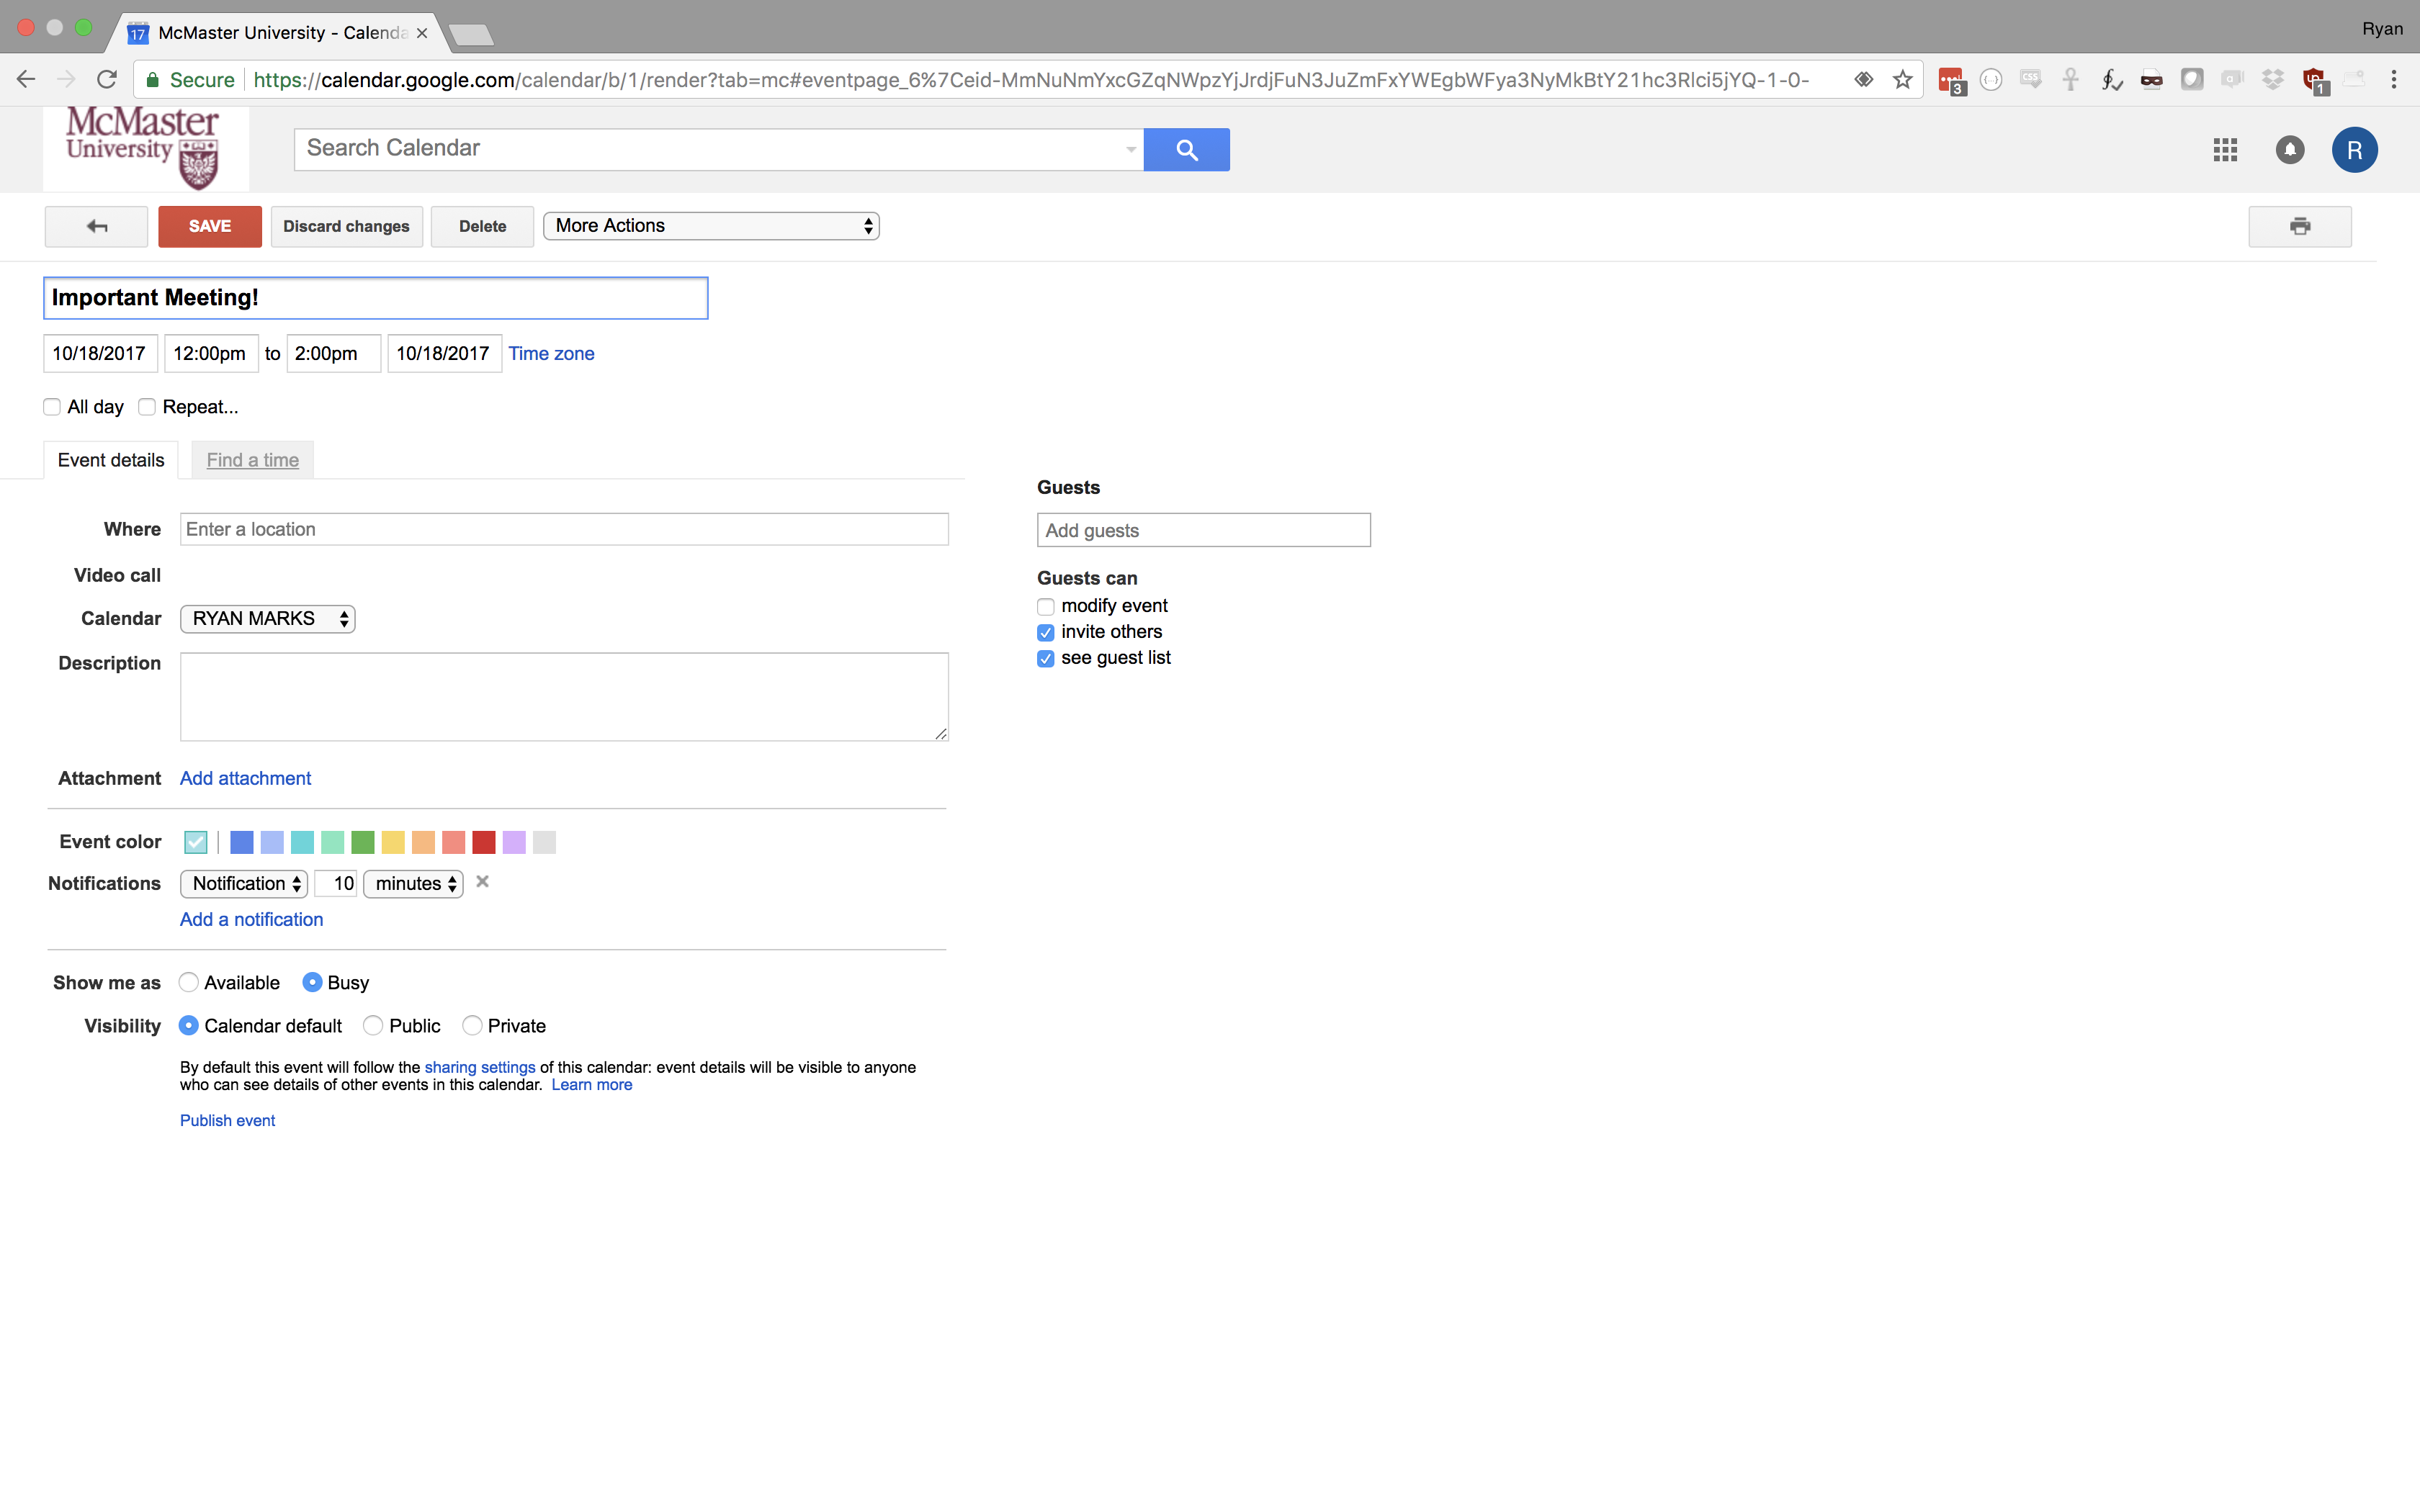
\includegraphics[width=\columnwidth]{{google/Invite2.1end}}
\caption{After subtask 2.1 of the invitation procedure for Google Calendar}
\end{figure}

\begin{figure}[H]
\centering
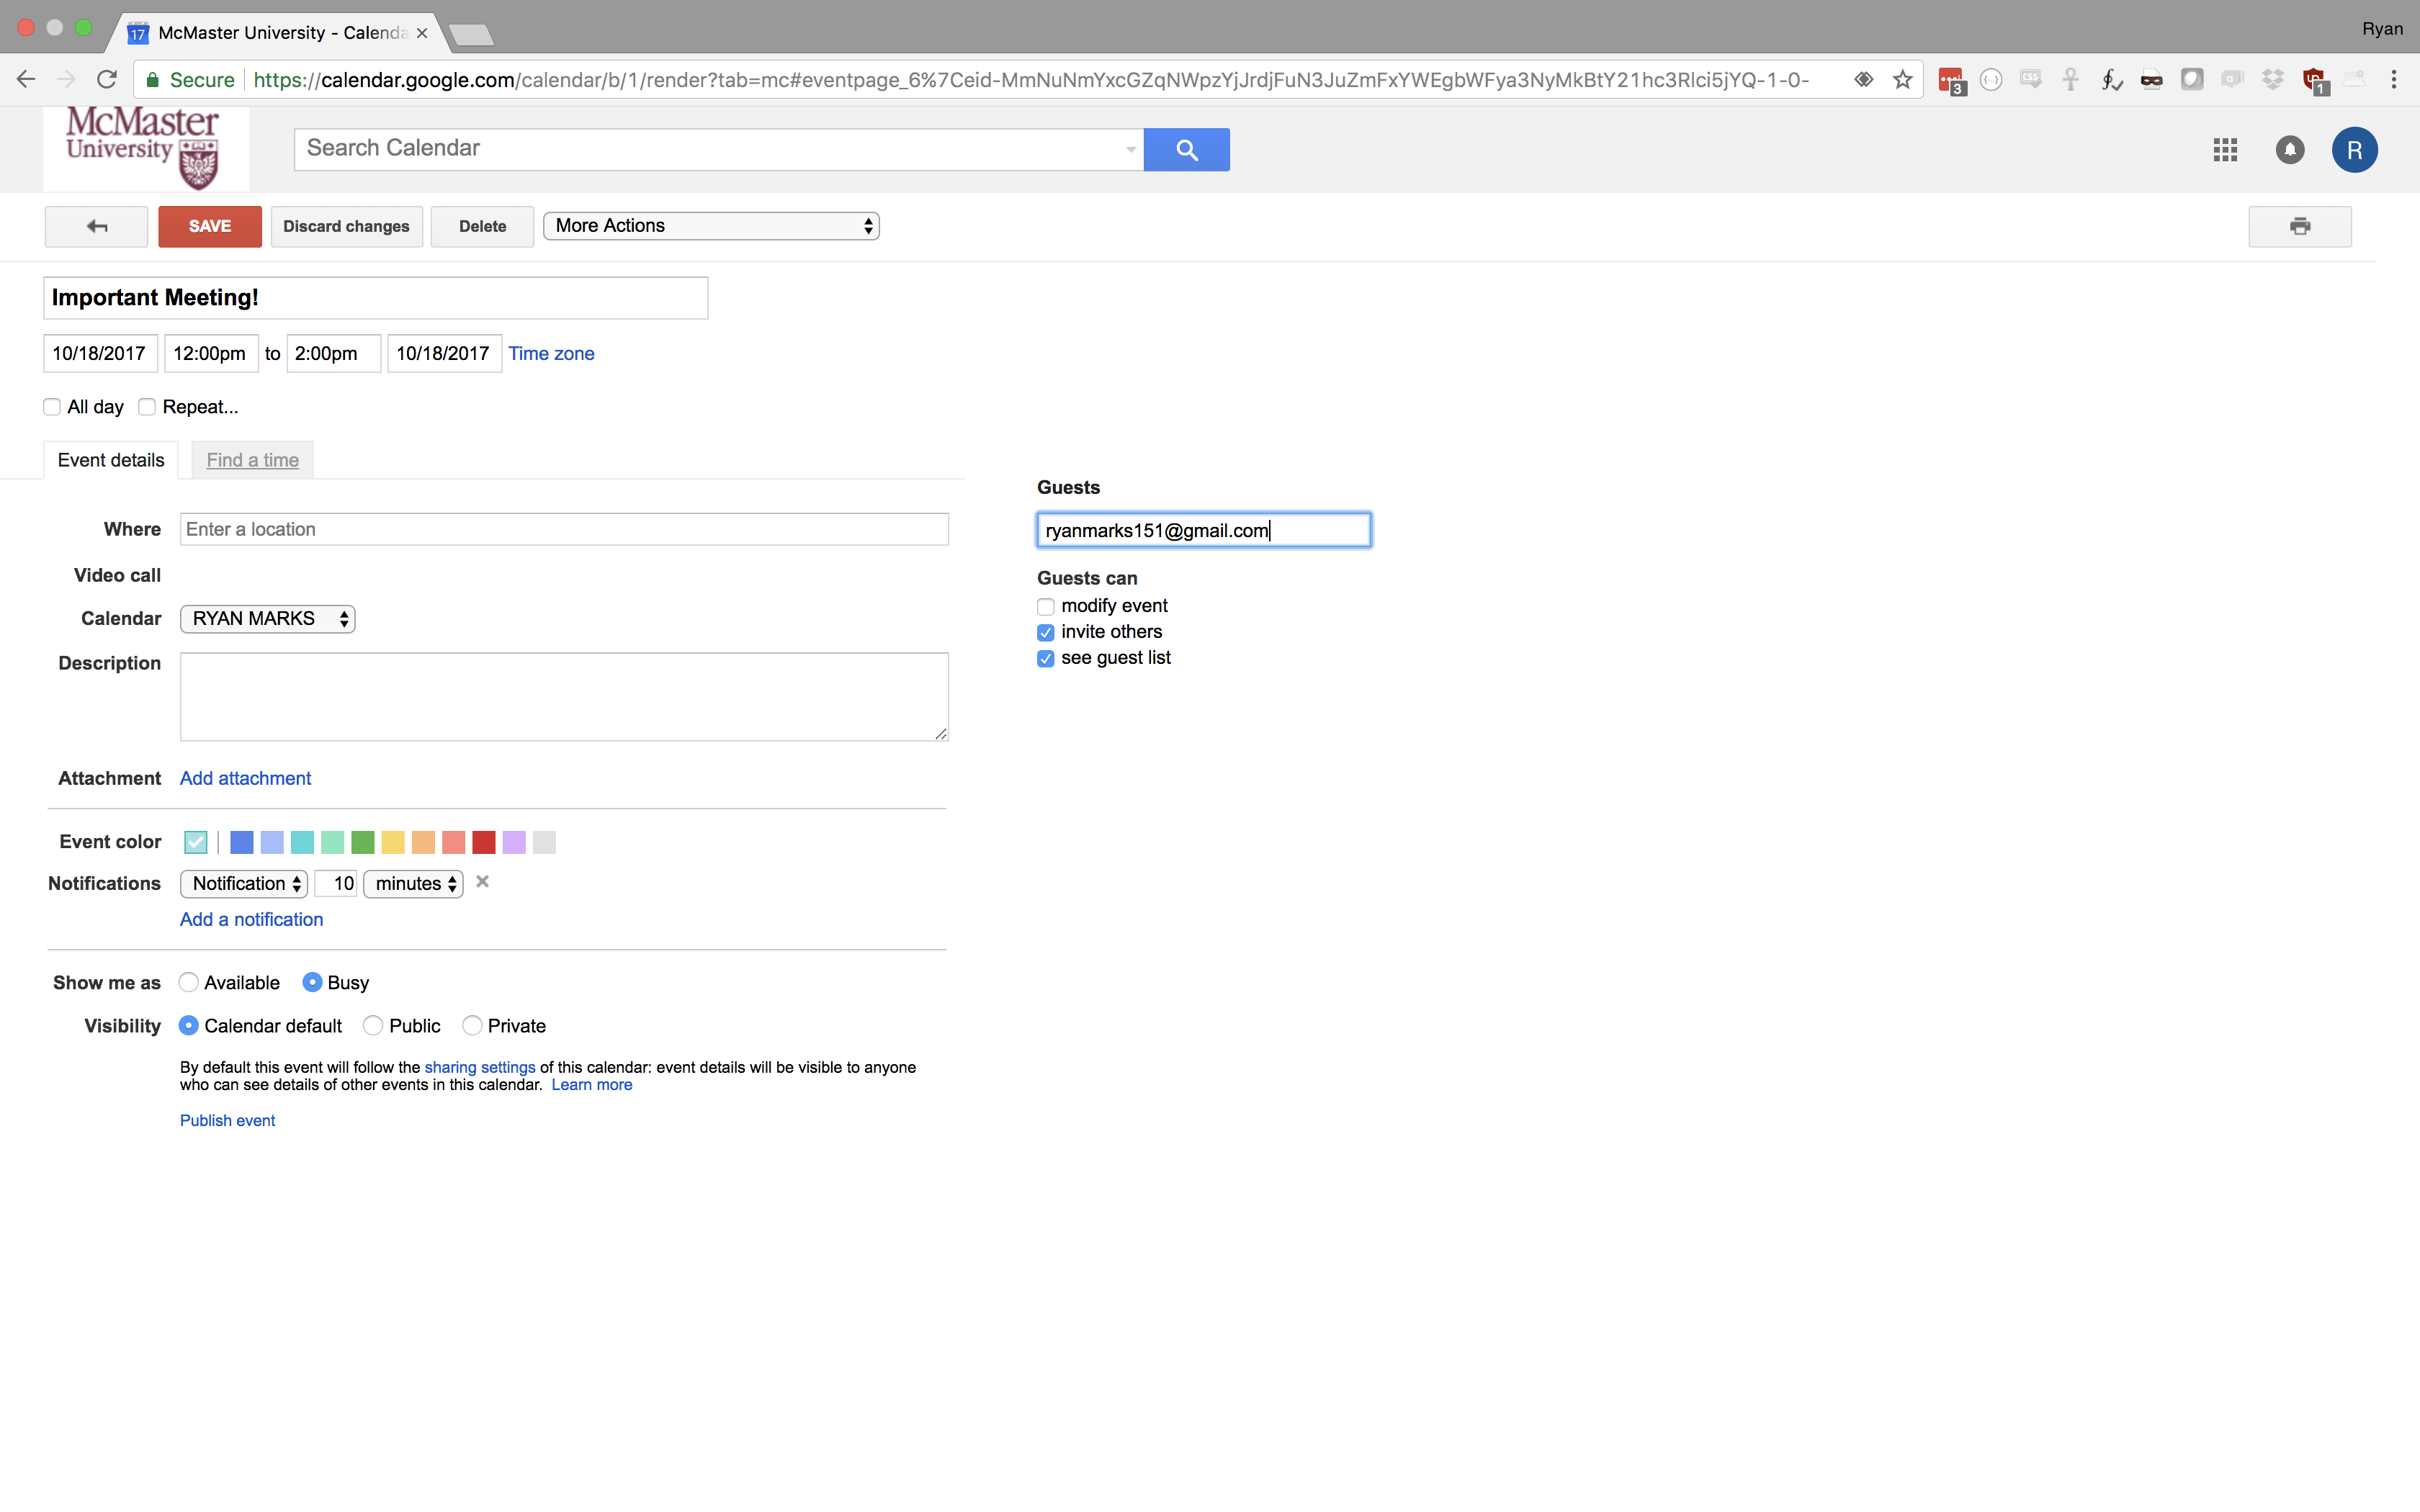
\includegraphics[width=\columnwidth]{{google/Invite2.2}}
\caption{Before subtask 2.2 of the invitation procedure for Google Calendar}
\end{figure}

\begin{figure}[H]
\centering
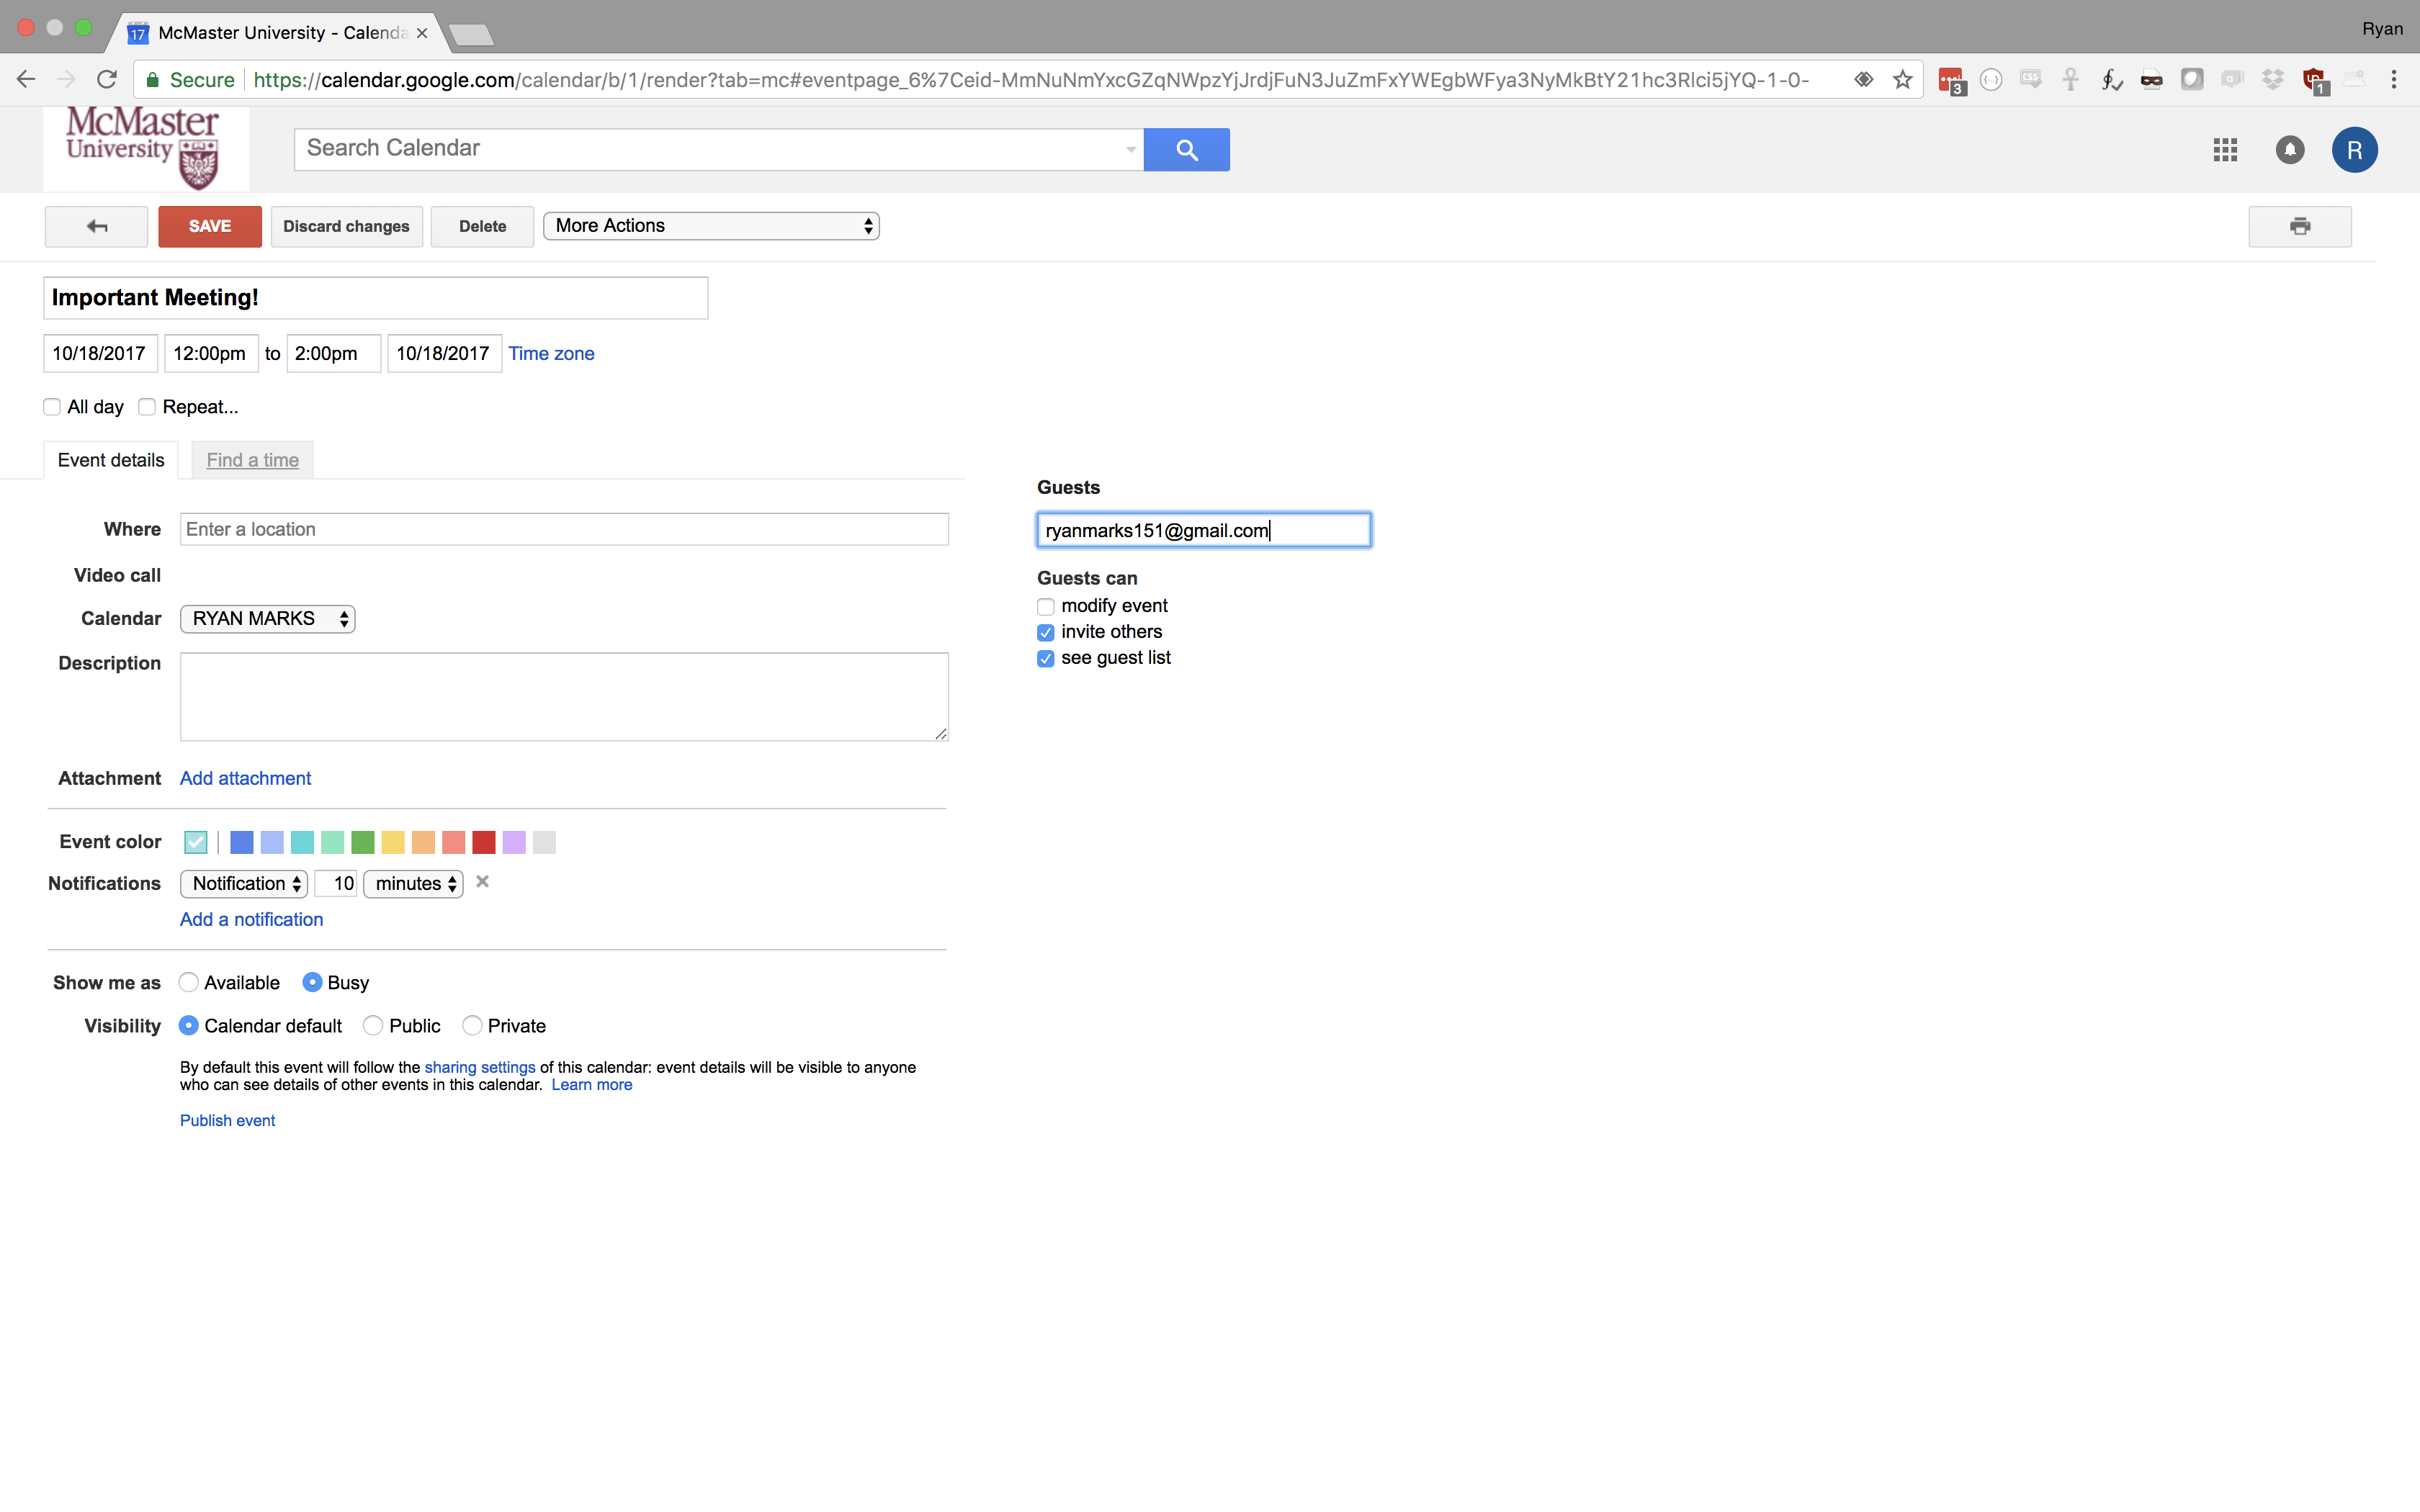
\includegraphics[width=\columnwidth]{{google/Invite2.2end}}
\caption{After subtask 2.2 of the invitation procedure for Google Calendar}
\end{figure}

\newpage

\begin{figure}[H]
\centering
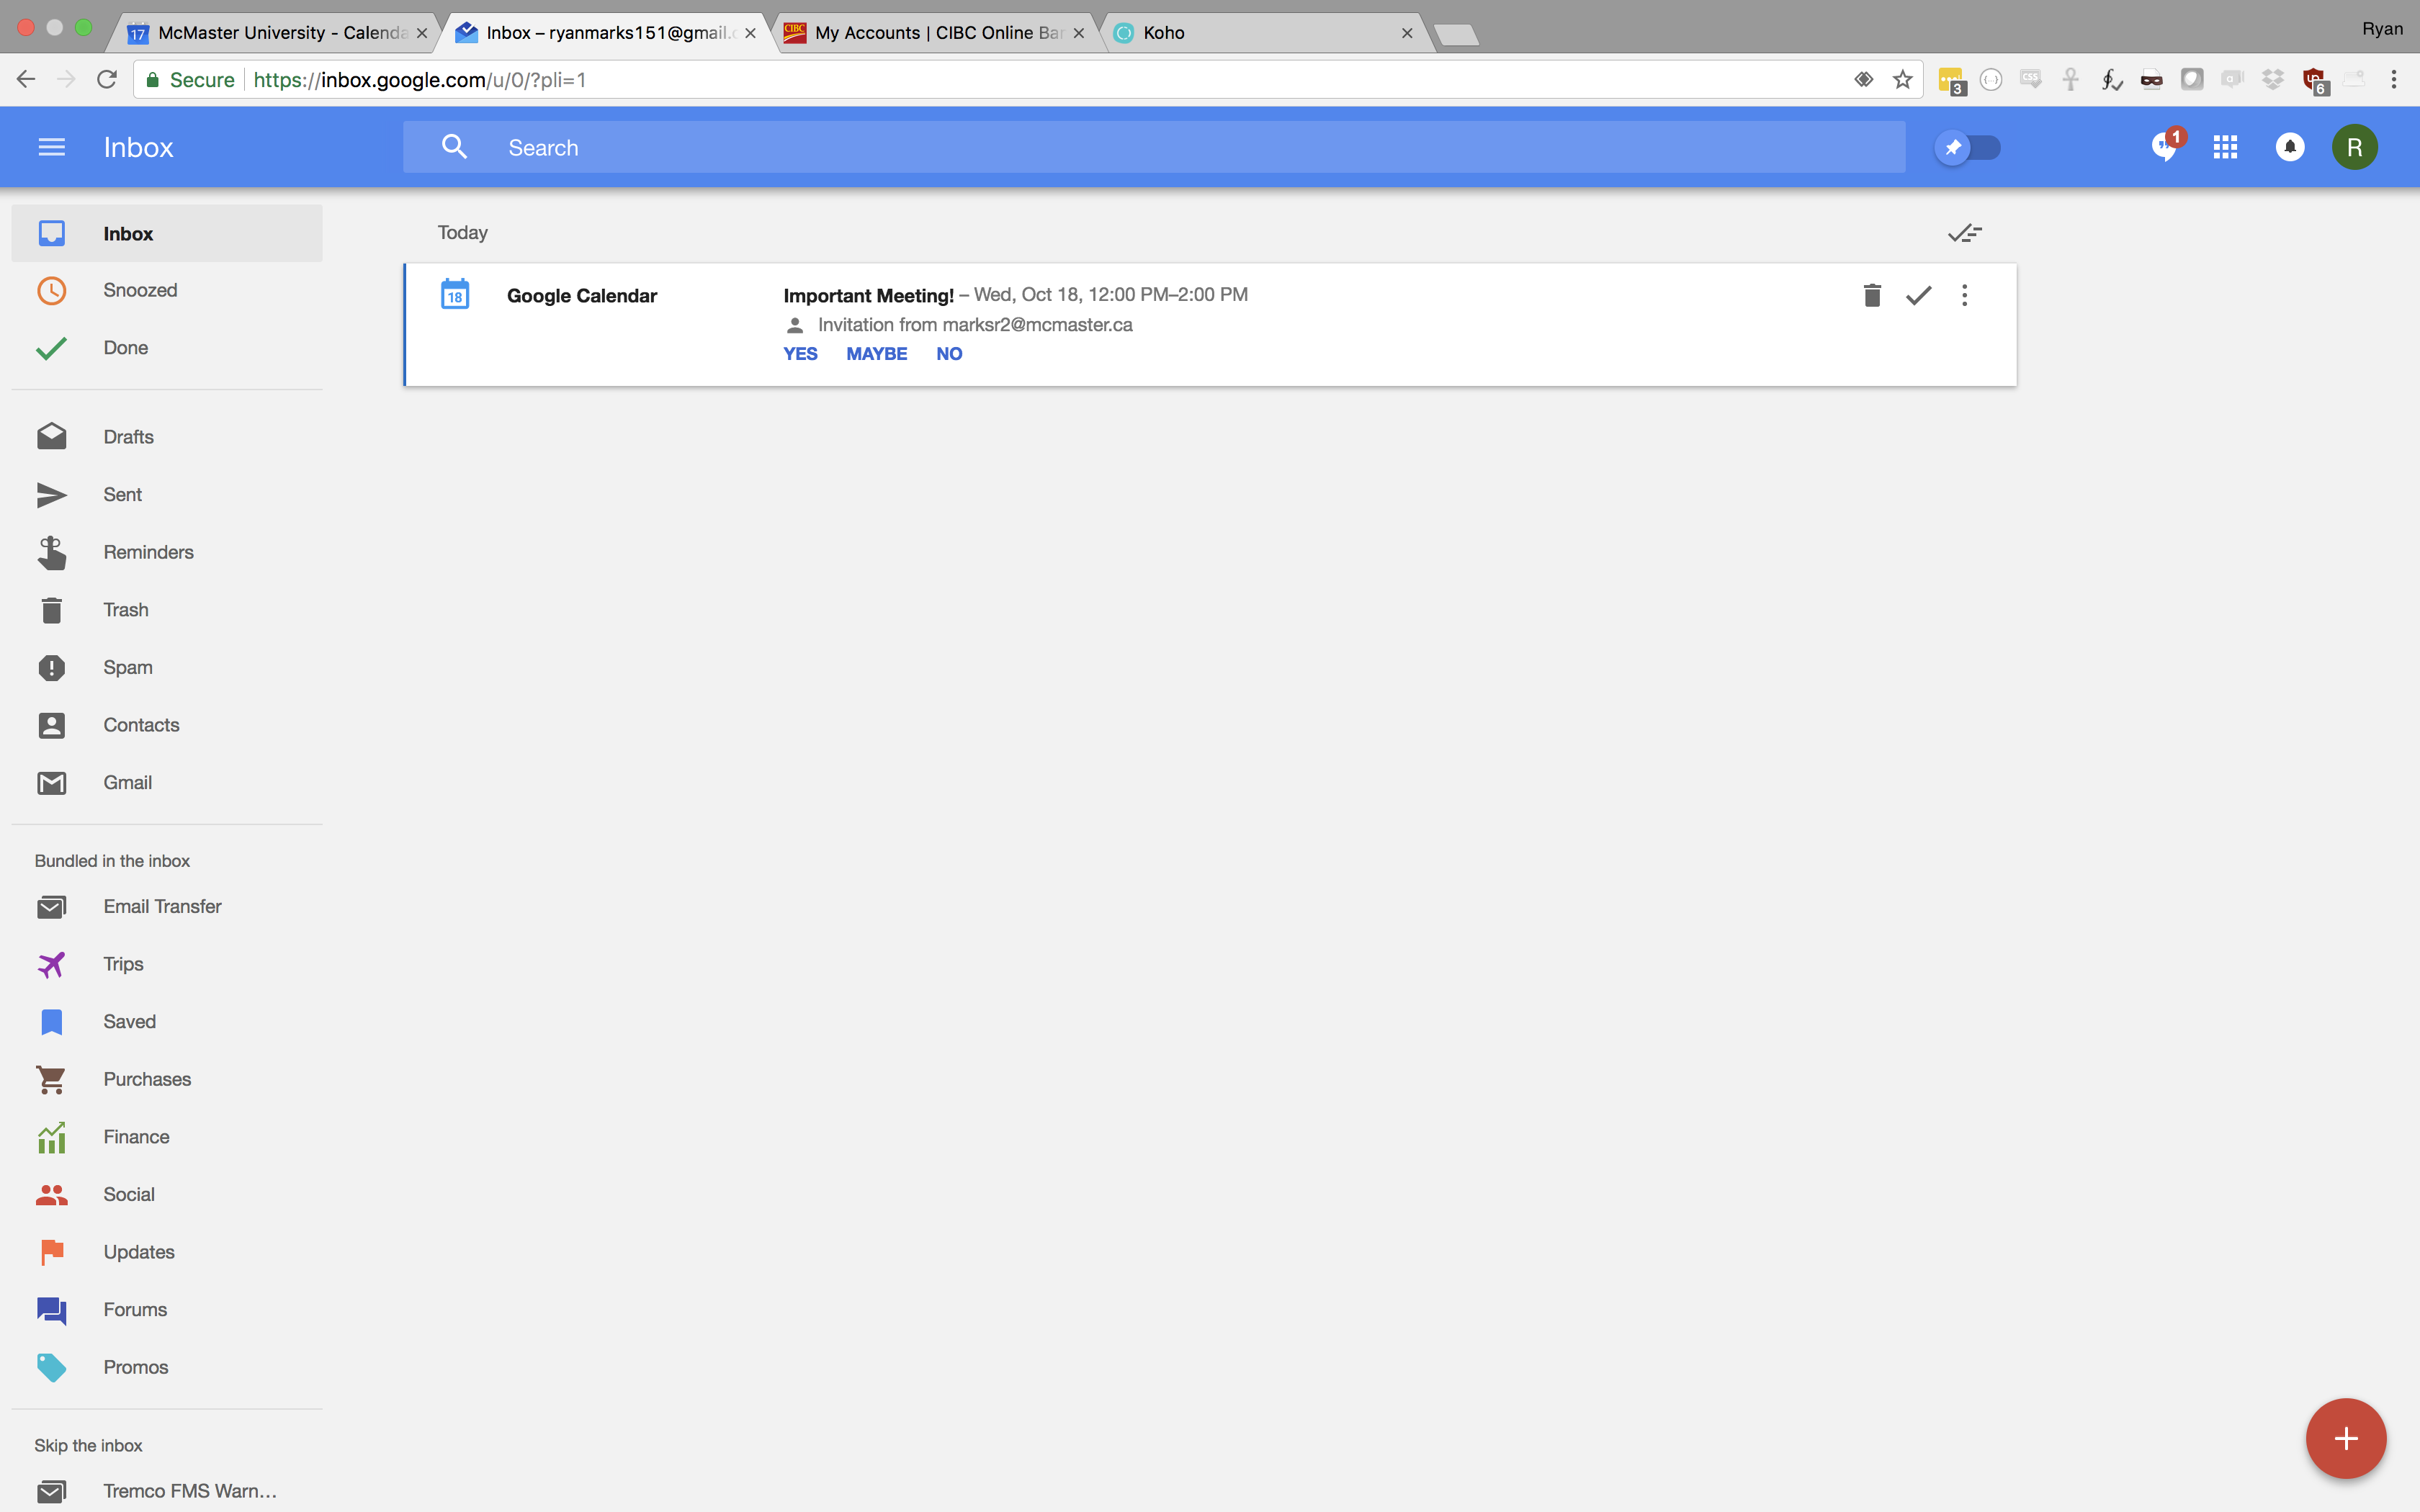
\includegraphics[width=\columnwidth]{{google/Respond1}}
\caption{Before subtask 1 of the invite response task with Google Inbox}
\end{figure}

\begin{figure}[H]
\centering
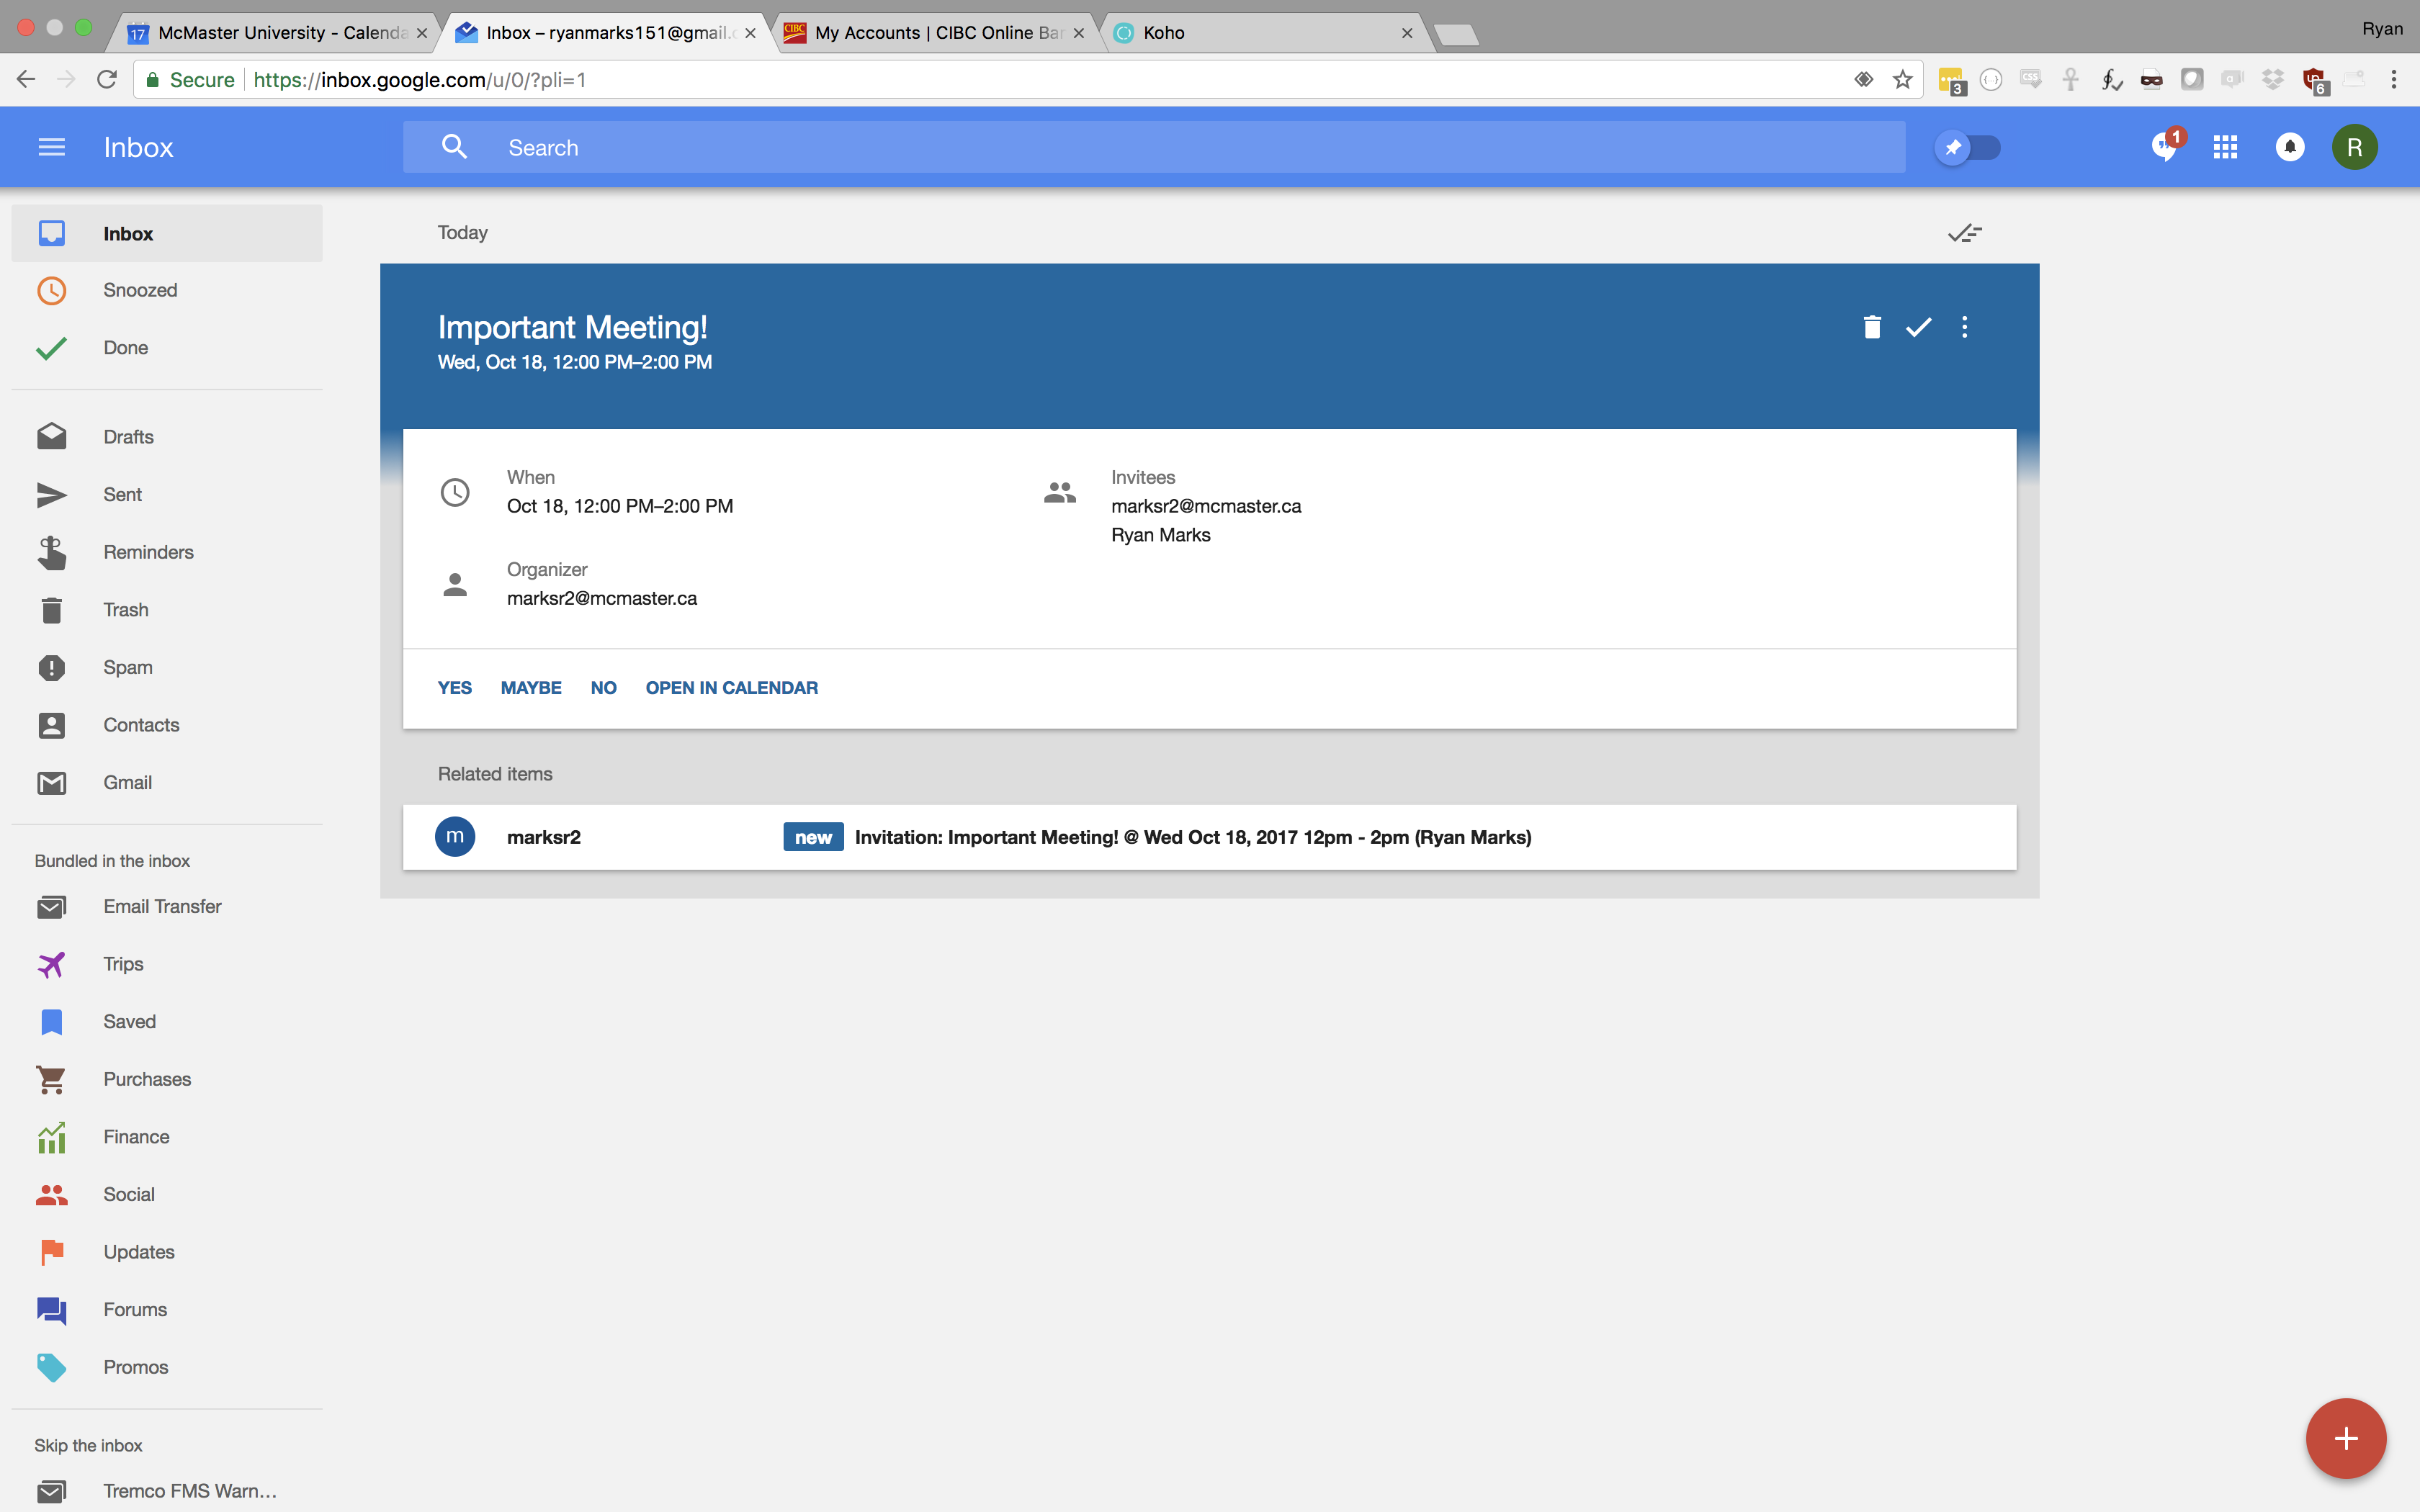
\includegraphics[width=\columnwidth]{{google/Respond1end}}
\caption{After subtask 1 of the invite response task with Google Inbox}
\end{figure}

\begin{figure}[H]
\centering
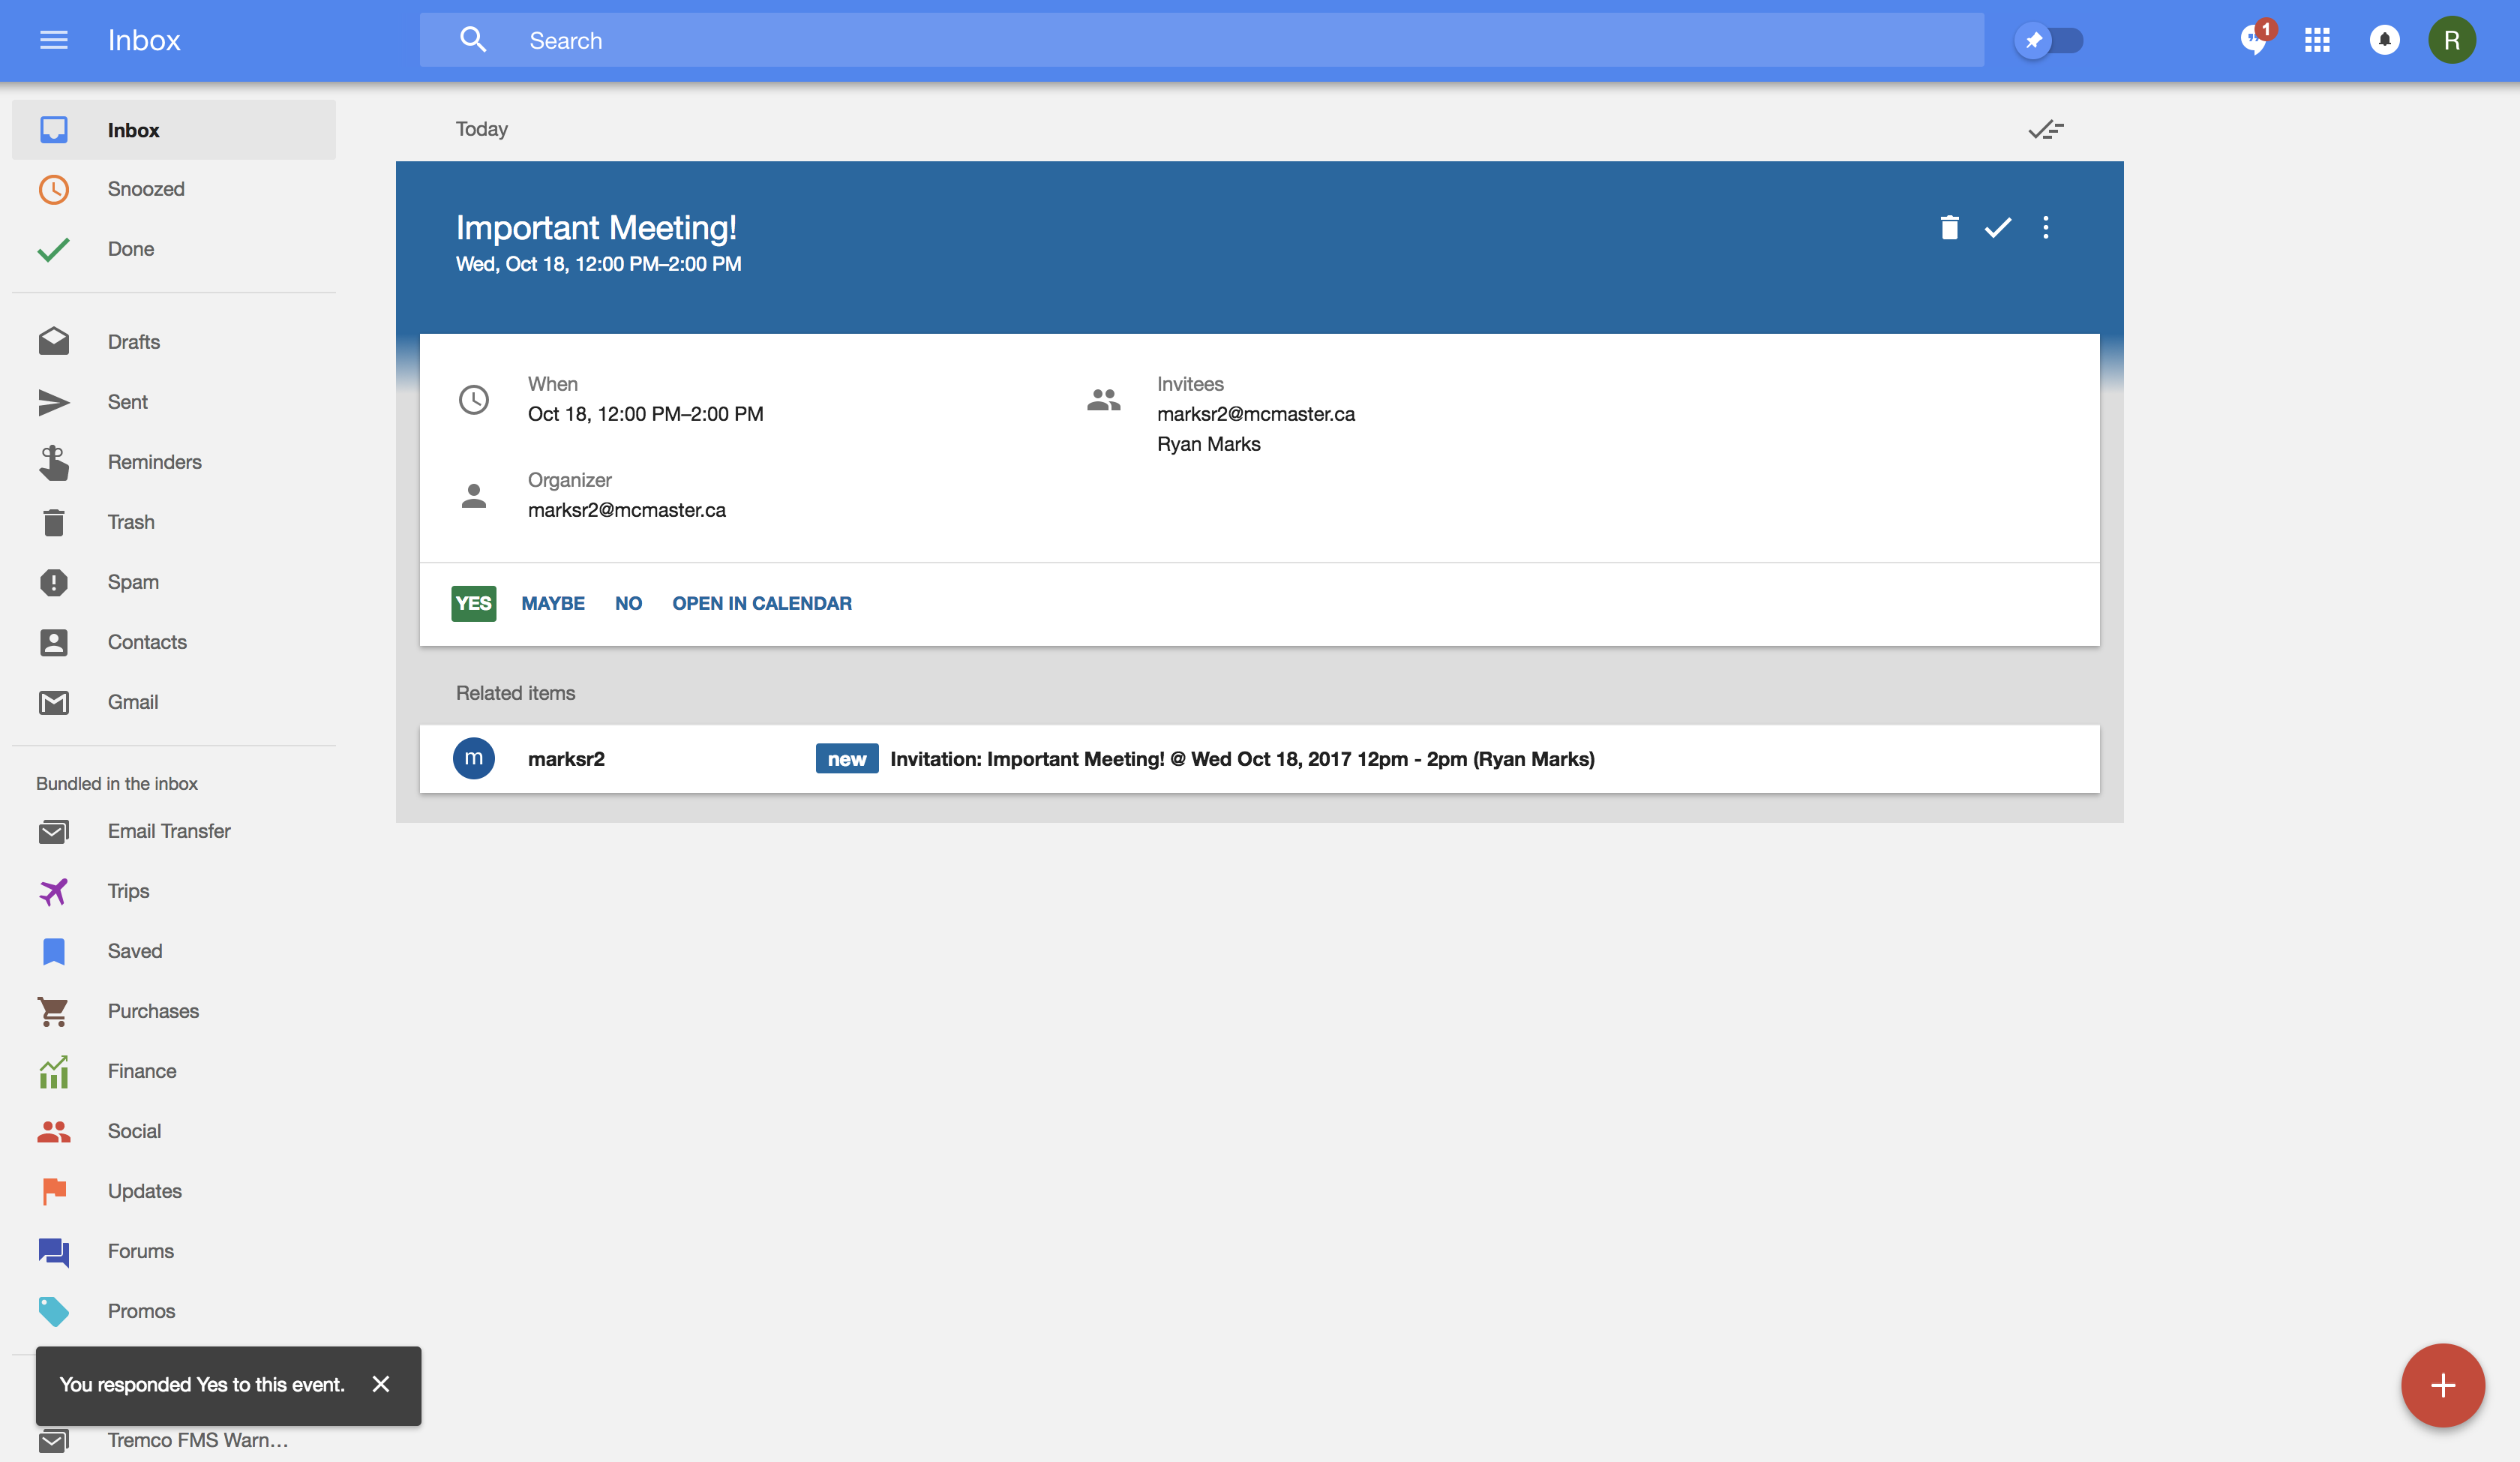
\includegraphics[width=\columnwidth]{{google/Respond2.1}}
\caption{Subtask 2.1 of the invite response task with Google Inbox}
\end{figure}


\begin{figure}[H]
\centering
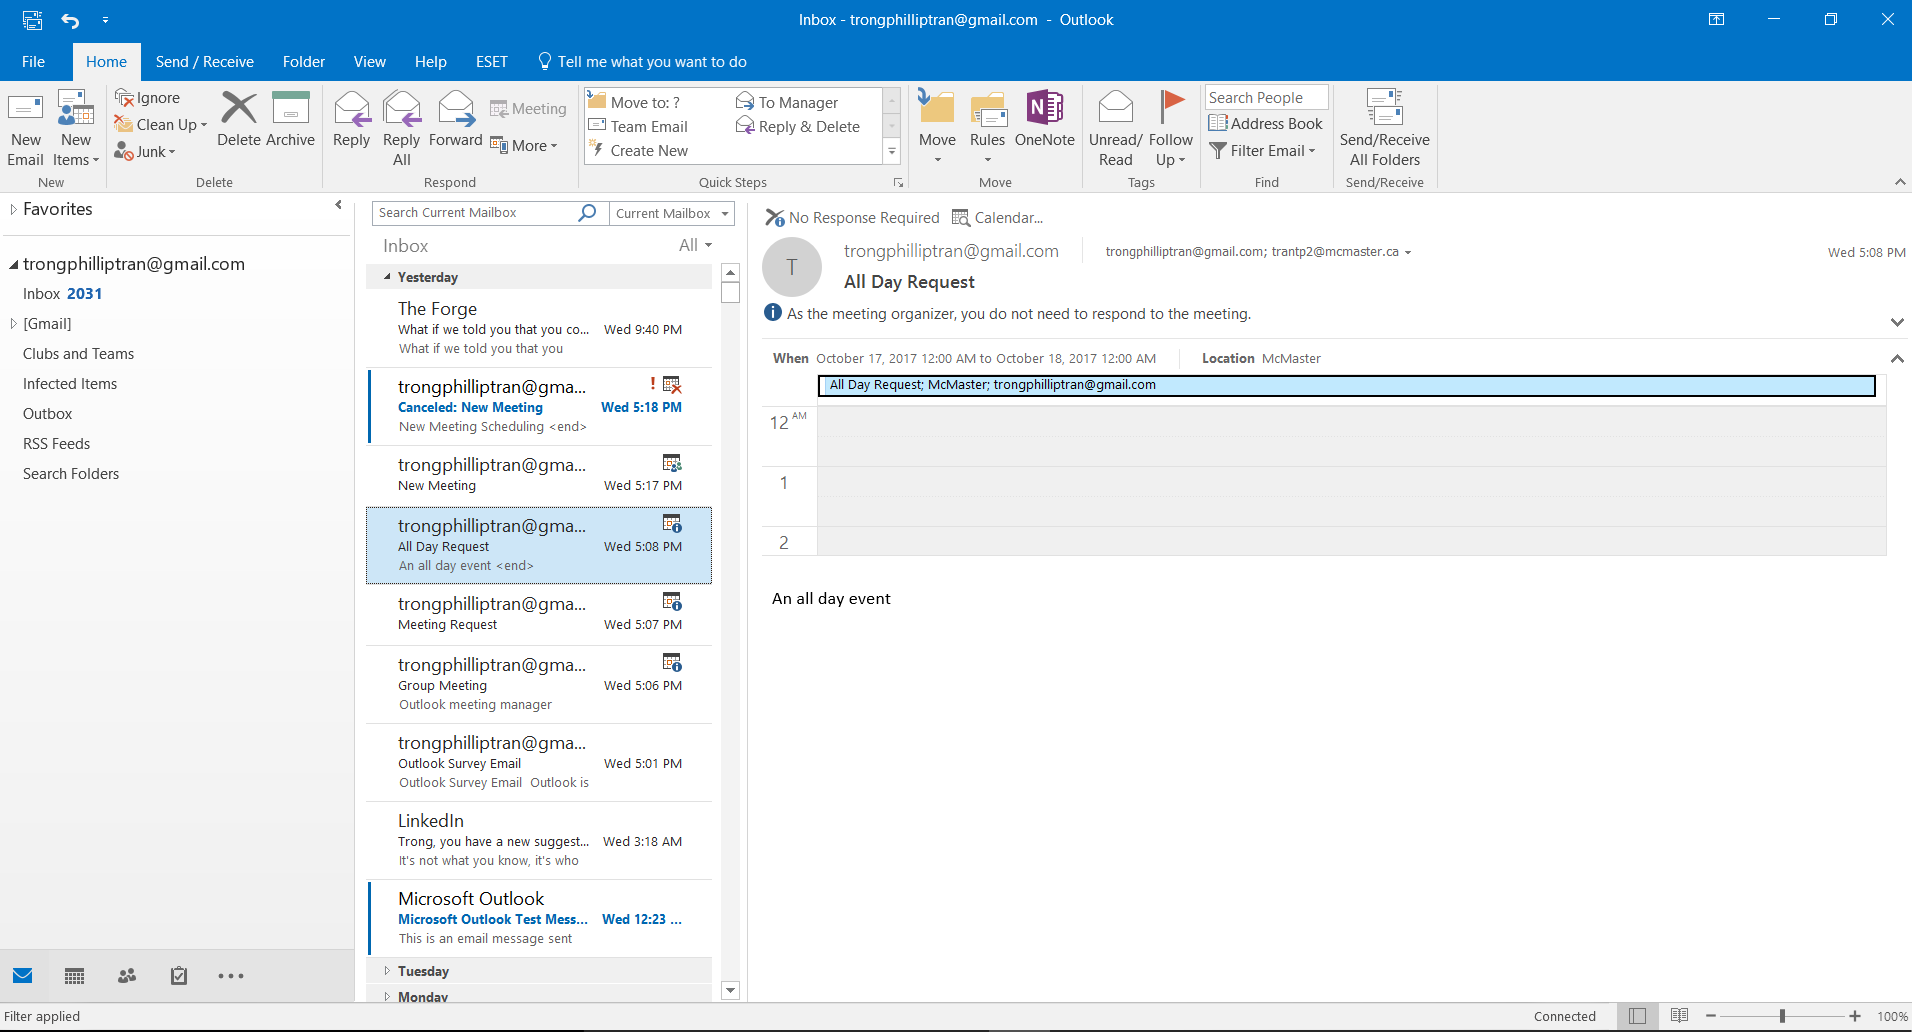
\includegraphics[width=\columnwidth]{{Outlook/Critique_Picture.png}}
\caption{Outlook has many options, which can be overwhelming if a user has no experience in using Microsoft Office type applications}
\end{figure}

\begin{figure}[H]
\centering
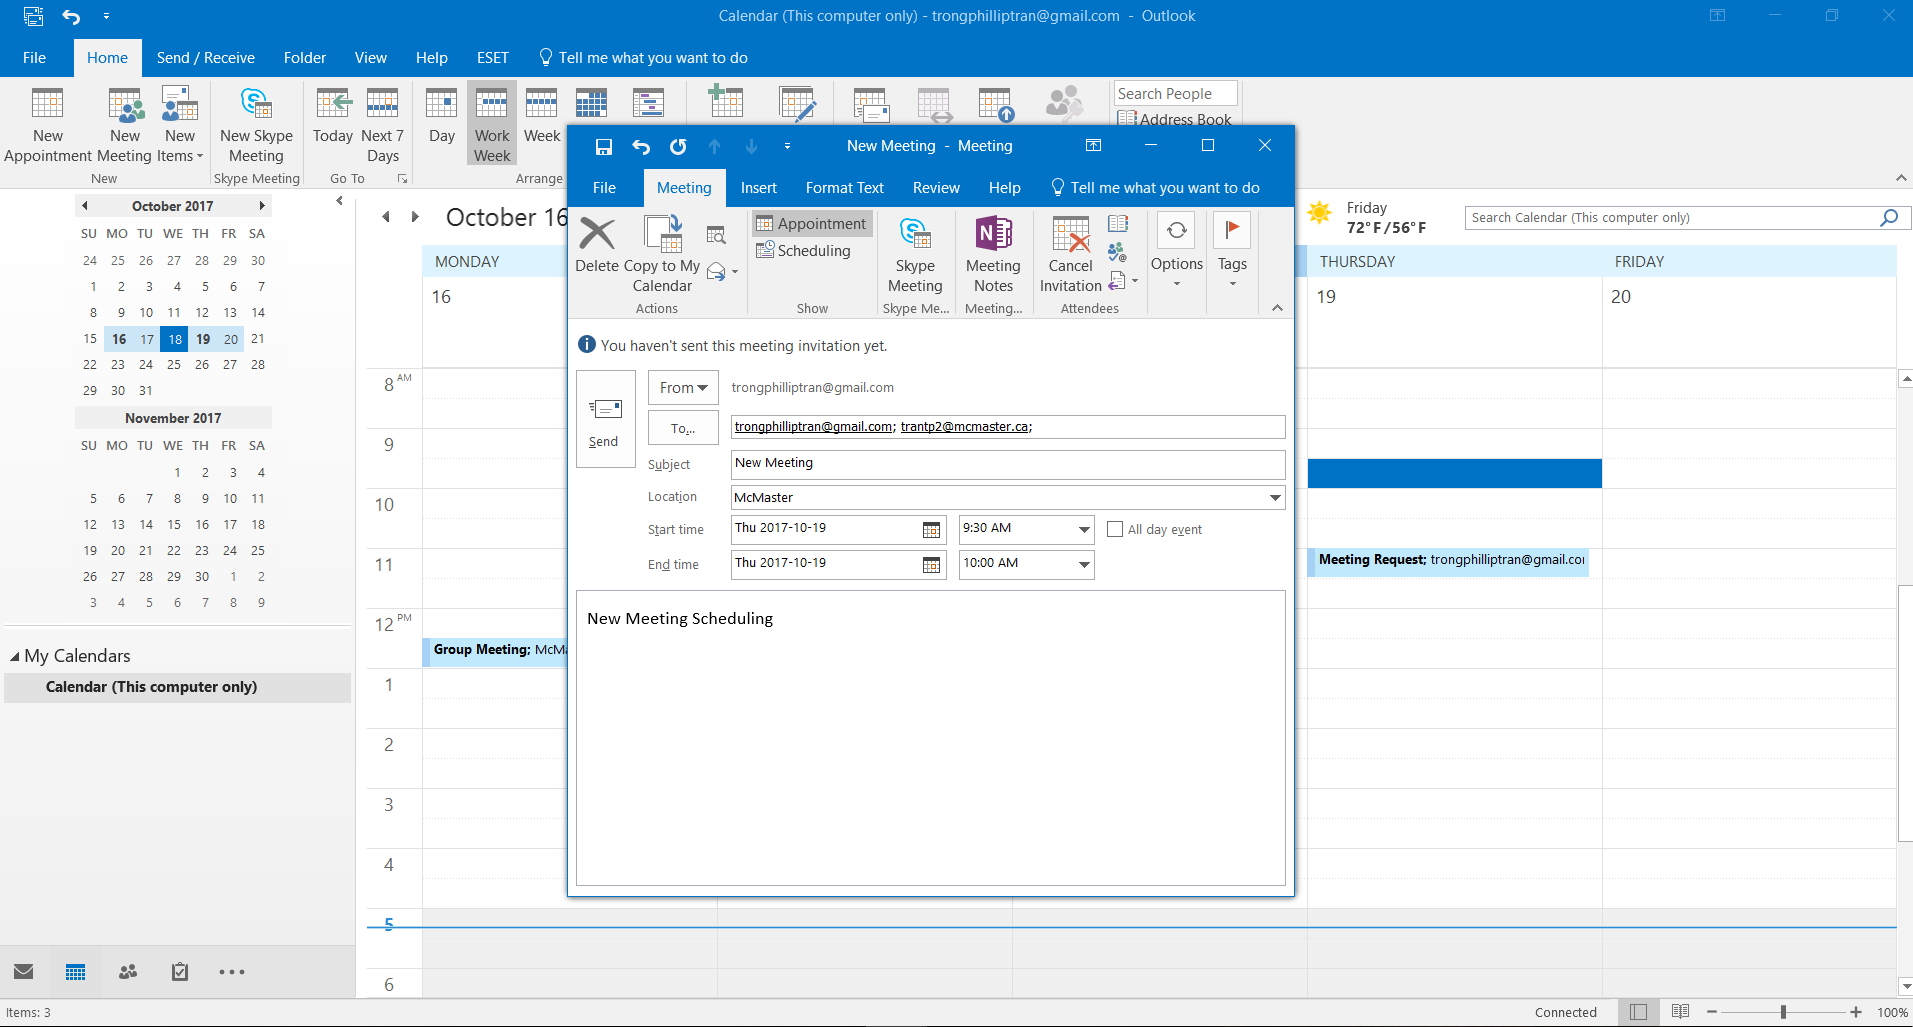
\includegraphics[width=\columnwidth]{{Outlook/New_Meeting_Schedule.png}}
\caption{New Meeting Scheduling}
\end{figure}

\begin{figure}[H]
\centering
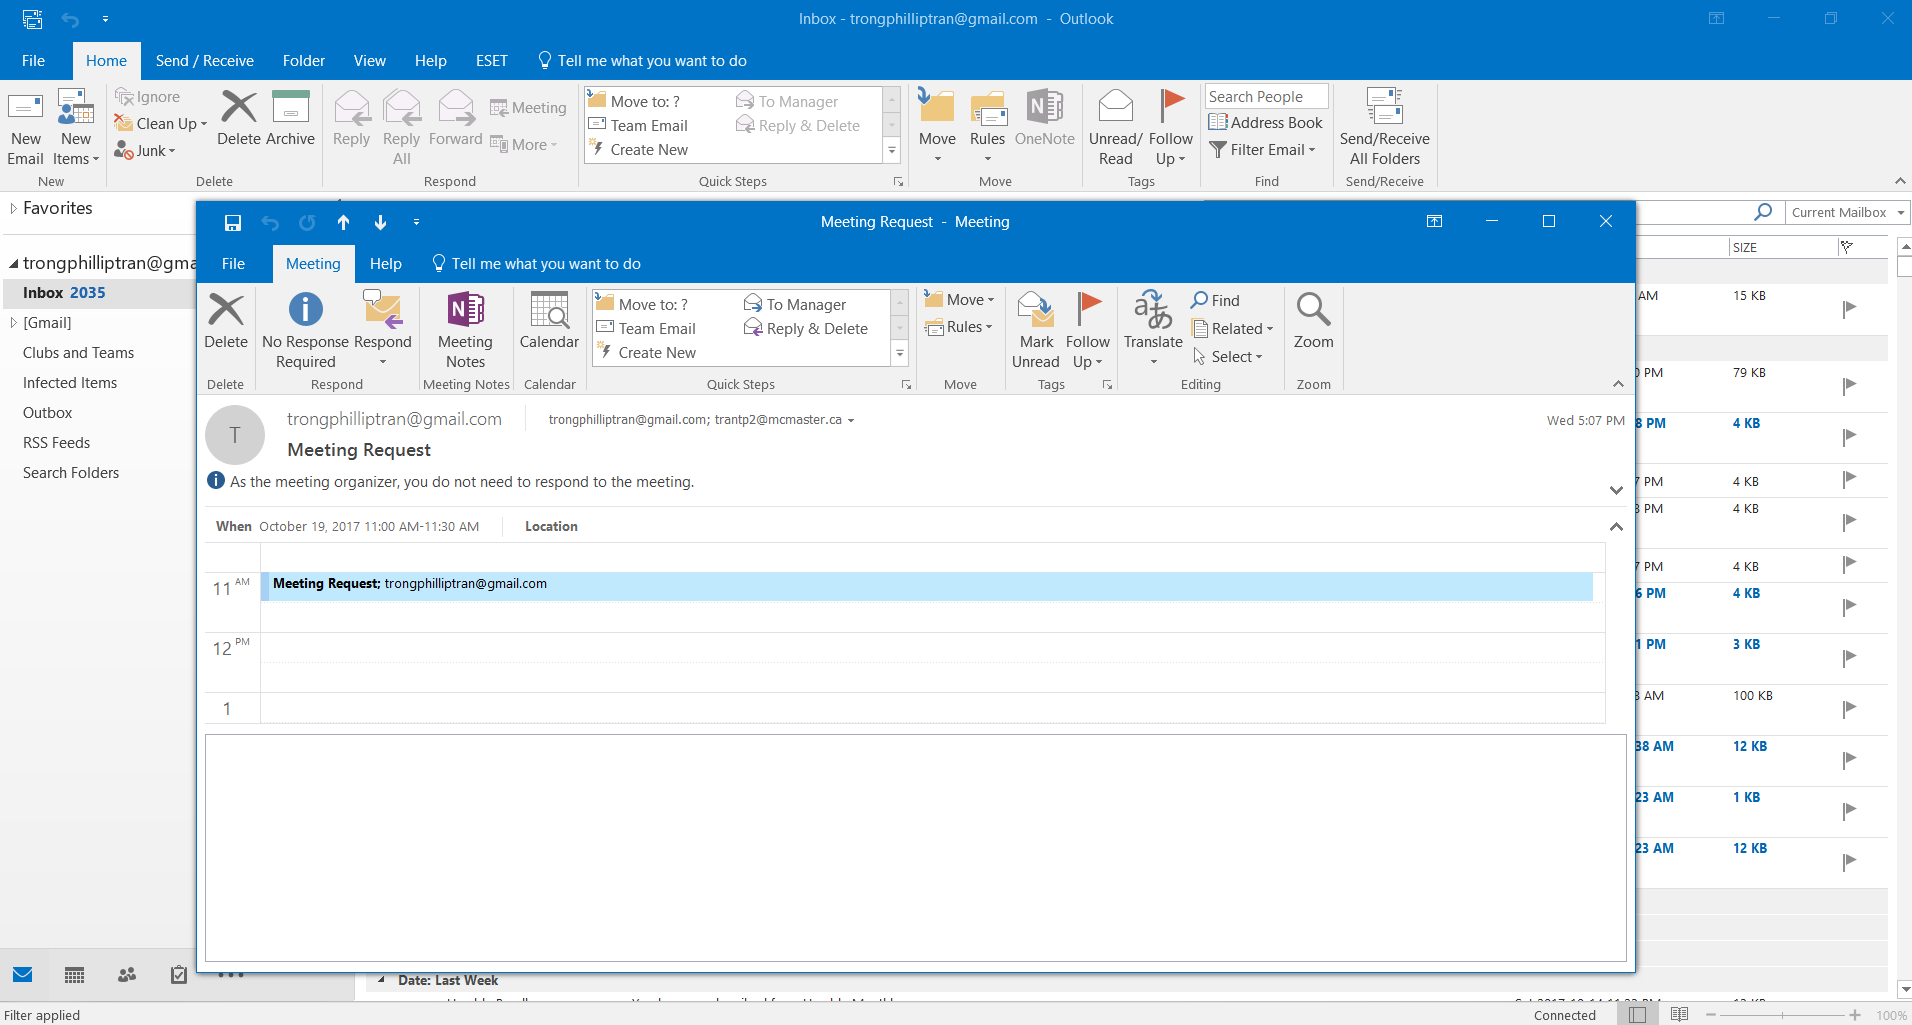
\includegraphics[width=\columnwidth]{{Outlook/Meeting_Request_Response.png}}
\caption{Meeting Request Response}
\end{figure}

\begin{figure}[H]
\centering
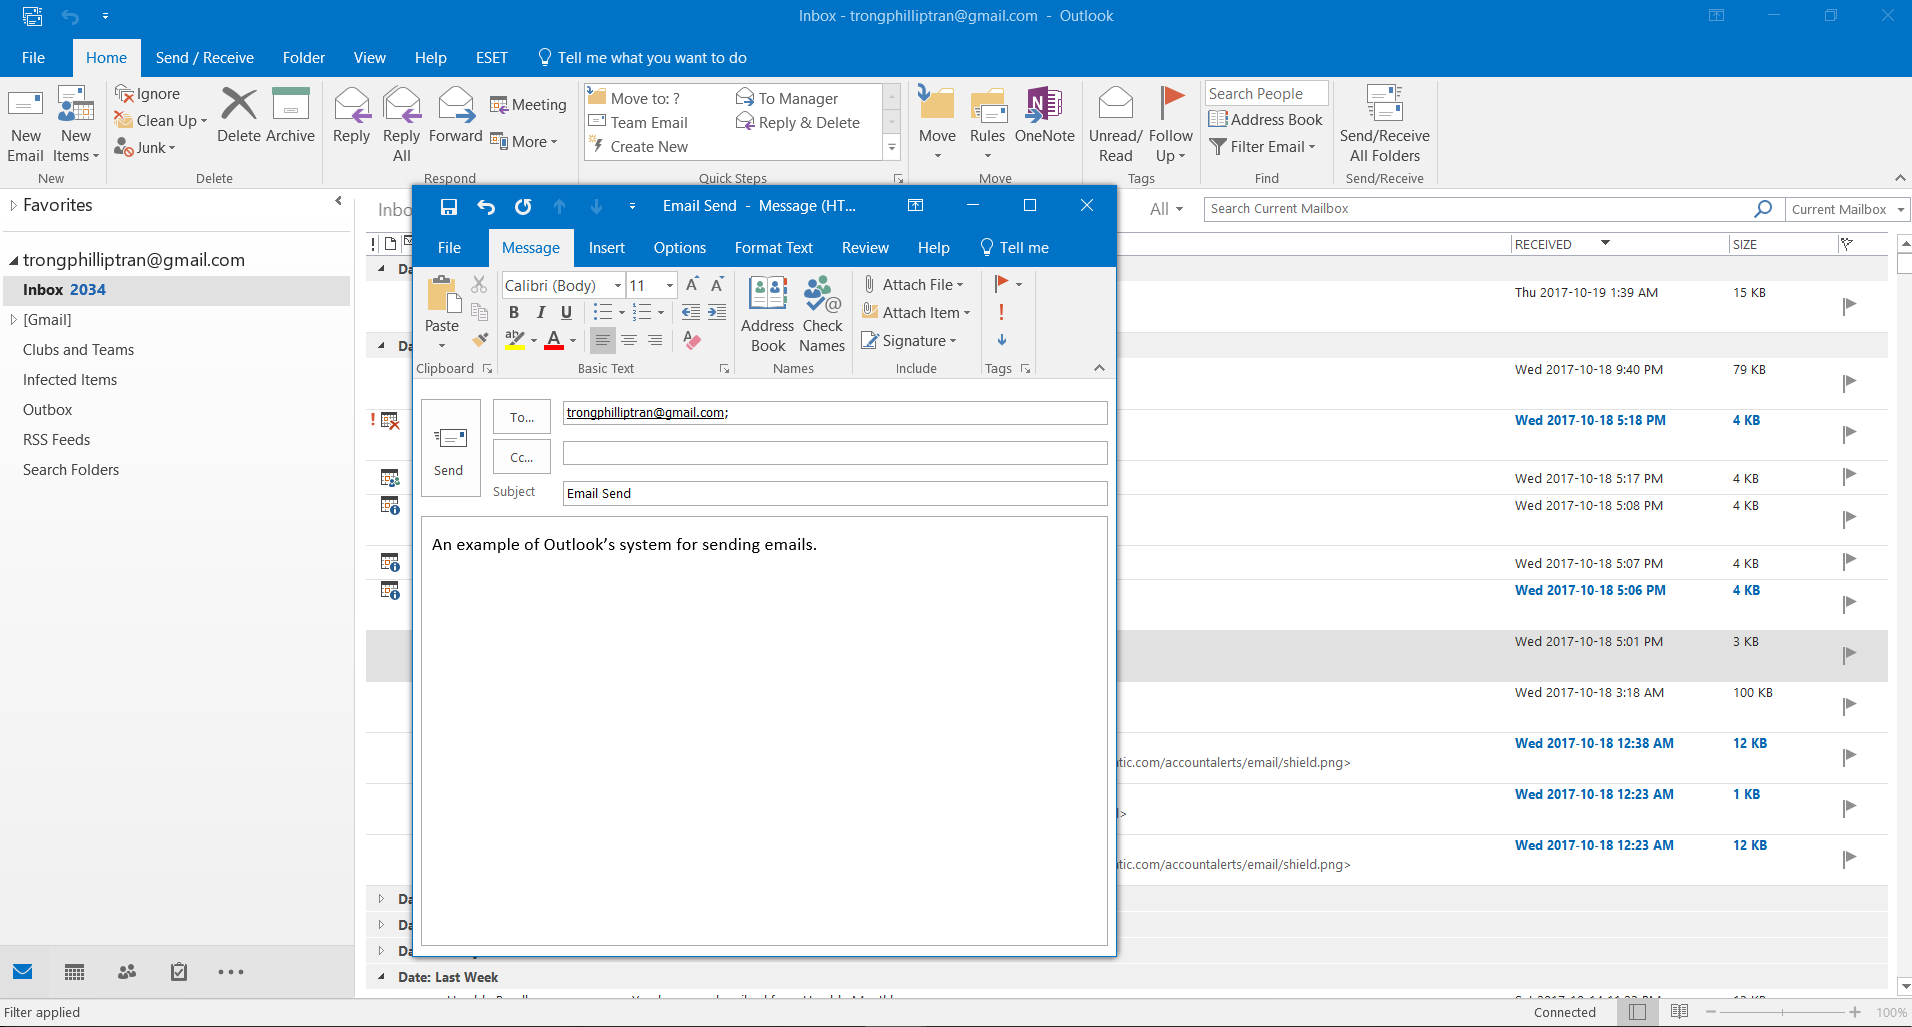
\includegraphics[width=\columnwidth]{{Outlook/Email_Send.png}}
\caption{Meeting Request Response}
\end{figure}

\begin{figure}[H]
\centering
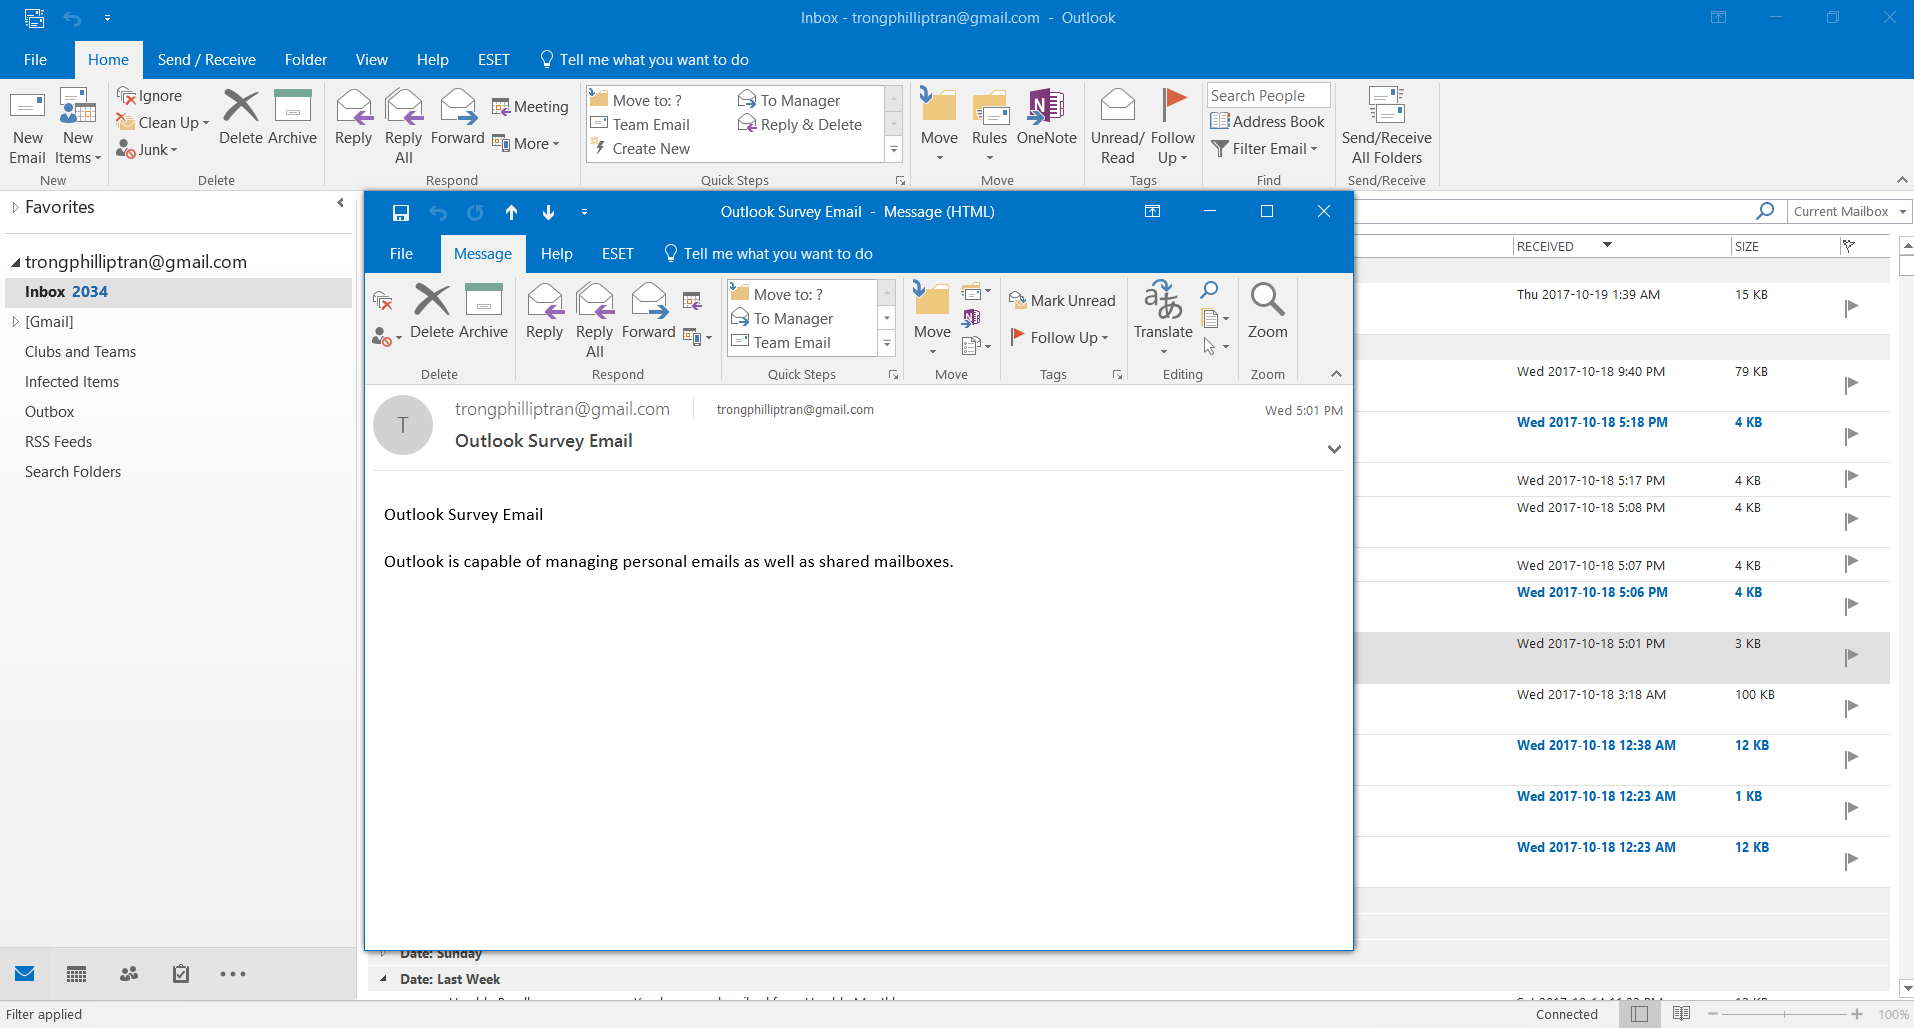
\includegraphics[width=\columnwidth]{{Outlook/Email_Reply.png}}
\caption{Meeting Request Response}
\end{figure}

\balance{}

\end{document}

%%% Local Variables:
%%% mode: latex
%%% TeX-master: t
%%% End:
